\documentclass[12pt]{article}


\usepackage[utf8]{inputenc}
\usepackage[margin=1in]{geometry}
\newgeometry{tmargin=1.5cm, bmargin=1.5cm, lmargin=1.5cm, rmargin=1.5cm}
% \usepackage[parfill]{parskip}

\usepackage{polski}
\usepackage[polish, english]{babel}
\usepackage{hyperref}
\usepackage{graphicx}
\usepackage{amsmath}
\usepackage[backend=biber,dateabbrev=false,sorting=none]{biblatex}
\addbibresource{bibliography.bib}
\usepackage[font=small, labelfont=bf, justification=justified]{caption}
\usepackage{titlesec}
\newcommand{\sectionbreak}{\clearpage}
% \usepackage[demo]{graphicx}
\usepackage{subcaption}
\usepackage{caption}
\captionsetup{justification=centering}
\usepackage{placeins}
\usepackage[table,xcdraw]{xcolor}

\title{Large Datasets Embedding and Visualization}
\author{Mateusz Smendowski, Michał Grela}
\date{June 2022}

\begin{document}

\maketitle

%%%%%%%%%%%%%%%%%%%%%%%%%%%%%%%%%%%%%%%%%%%%%%%%%%%%%%%%%%%%%%%%%%%%%%%%%%%%%%%%%%%%%%%%%%%%%%%%%%%%%%%%
\section{Introduction}
Visualization makes it easier to understand and notice dependencies in the high dimensionality data that are not trivial to capture and perceive. It is an inseparable, far-reaching, and effectual concept of data analysis or its initial recognition, but also an autonomous tool and dextrous field of machine learning. Visualization allows checking whether there are groups of similar observations forming clusters and finally gain more priceless intuition and understanding about data. In the case of multi and high-dimensional ones, it is necessary to reduce their dimensions to at most three. The relationships in data are often non-linear, which rules out methods like PCA regarding separation quality (Figure 1). Therefore, it is required to use Manifold Learning techniques to discover the surface (manifold) on which the data is distracted and make reasonable projections into a space with the desired dimensionality.

\begin{figure}[h]
    \centering
    \includegraphics[width=0.5\textwidth]{manifold_projection.png}
    \caption{Comparison of PCA projection with manifold learning techniques..}
    \label{fig:mnist_visualization}
\end{figure}

This project aims to analyze and visualize the MINST, 20 News Groups, and RCV Reuters datasets using methods such as t-SNE, UMAP, ISOMAP, PaCMAP and IVHD. Therefore, the particular motivation is to show the concept of high-dimensional data visualization, assess multiple data embedding techniques, and highlight potential comparative criteria of data separation quality. This document is organized as follows: Section 2 introduces the used data sets. Subsequently, Section 3 includes theoretical descriptions of applied dimensionality reduction techniques and implemented metrics. The next part consists of visualizations and metric computations results. Finally, Section 5 states a space for a summary and conclusions.

\section{Datasets description}
In this section, analyzed datasets: MNIST, 20 News Groups and RCV Reuters are described.
\subsection{MNIST}
The MNIST (Modified National Institute of Standards and Technology database) dataset consists of the 70 000 size-normalized and centered images of hand-written digits (written by 500 different writers), where 60 000 samples make up the training set \cite{mnist_description}. Typically, the remaining collection intends for testing. More specifically, the MNIST is a subset of a larger NIST dataset with a 28x28 size and black and white images of digits, which is a benchmark set not only for classification assessment but also for evaluating multiple methods of dimensionality reduction. Its great advantage is interpretability and intuitiveness. Because an average person can assess which of the digits are similar, it is possible to verify the data embedding techniques methods in terms of global separation and the reasonableness of the clusters created. Natural intuition suggests that representations of analogous digits such as 3 and 8 should be next to each other in the visualized space after dimensionality reduction. The size of the data set is 128 MB.

\begin{figure}[h]
    \centering
    \includegraphics[width=0.6\textwidth]{mnist_digits.png}
    \caption{Visualization of sample digits from the MNIST data set.}
    \label{fig:mnist_digits_visualization}
\end{figure}

\subsection{20 News Groups}
The 20NG (20 News Groups) dataset consists of 18 846 posts from 20 news groups \cite{scikit_tng}. Each post has a representation in the form of a TF-IDF 5000-word vector. The extracted TF-IDF vectors are very sparse, with an average score of less than .5\% non-zero features. Furthermore, the collection includes 20 classes associated with thematic areas such as graphics, baseball, and electronics. Finally, the size of the entire data set is around 413 MB.

\subsection{RCV Reuters}
The RCV (Reuters Corpus Volume) Reuters dataset consists of 804 409 manually classified news \cite{rcv_description}. The original dataset includes 103 classes and 47 236 dimensions. We have operated on its minimized version with attributes reduced to 30 via PCA (corpus of press articles preprocessed to 30D by PCA). Our investigation proved that exactly 59 documents have less or equal to 200 samples. In order not to introduce the phenomenon of noise that could significantly obscure and deteriorate the quality of the visualization, small classes have been removed, leaving the content of 24 unique documents. Consequently, the ultimate size of the data set occurred to be around 235 MB.

\clearpage
\section{Used methods}
In this section, used embedding methods and metrics to measure their quality are briefly described.
\subsection{Embeddings}
An embedding is a low-dimensional representation of high-dimensional data. Usually, it is impossible to fully map the structure of multidimensional data, but it is possible to map that is sufficient to solve a given problem. Many methods have been developed for data embedding. In this subsection, theoretical aspect of used embedding methods is presented. It is recommended to read the original papers and documentations to fully understand the issues presented in this subsection.
\subsubsection{t-SNE}
t-Distributed Stochastic Neighbor Embedding (t-SNE) was first proposed by Laurens van der Maaten and Geoffrey Hinton in 2008\cite{vanDerMaaten2008}. t-SNE is a variant of the Stochastic Neighbor Embedding (SNE), so in order to understand how t-SNE works it is necassary to introduce SNE method\cite{HintonRoweis2003}. The method starts by finding the similarities between neighboring objects in high-dimensional space, which is determined by the conditional probability $p_{i|j}$ given by
\begin{equation}
\label{eq:sne_prob_hd}
    p_{i|j}=\frac{\exp(-||x_{i}-x{j}||^{2}/2\sigma_{i}^2)}{\sum_{k\neq i}\exp(-||x_{i}-x_{k}||^2/2\sigma_{i}^2)}
\end{equation}
where $\sigma_{i}$ is either found by binary search for the value of it that gives probability distribution with a perplexity specified by the user or is set by hand. Whereas, in  the low-dimensional space Gaussian neighborhoods are also used, but with a specified variance value set to $\frac{1}{2}$. So the conditional probability $q_{i|j}$ that object $i$ picks $j$ as its neighbor is given by the expression
\begin{equation}
\label{eq:sne_prob_ld}
    q_{i|j}=\frac{\exp(-||y_{i}-y{j}||^{2})}{\sum_{k\neq i}\exp(-||y_{i}-y_{k}||^2)}
\end{equation}
In the SNE method, the cost function is defined as sum of Kullback-Leibler divergences between distributions given by
\begin{equation}
\label{sne_cf}
    C=\sum_{i}\sum_{j}p_{i|j}\log\frac{p_{i|j}}{q_{i|j}}
\end{equation}
However classic SNE has two main problems. First, it is based on a cost function that is difficult to optimize. Second, it encounters a problem called "crowding problem", which is caused by Gaussian "short tail". In order to solve this problem, t-SNE uses the Student's t-distribution with a single degree of freedom, which is heavy-tailed distribution. So in t-SNE probability $q_{ij}$ is given by
\begin{equation}
\label{eq:tsne_prob_ld}
    q_{i|j}=\frac{(1+||y_{i}-y_{j}||^2)^-1}{\sum_{k\neq l}(1+||y_{k}-y{l}||^2)^-1}
\end{equation}
Despite the fact that t-SNE gives quite good results, this method also has its disadvantages. First, it is sensitive to the curse of the intrinsic dimensionality of the data, due to its local nature. The second, which is the major problem of this method, is the necessity to select several optimization parameters as the cost function is not convex.

\subsubsection{UMAP}

Uniform Manifold Approximation and Projection (UMAP) is a modern technique for dimension reduction developed by Leland McInnes, John Healy, James Melville in 2018\cite{McInnesHealyMelville2018}. It is characterized by faster run time and better preservation of the global structure of data than t-SNE. The UMAP is based on three assumptions about the data:
\begin{enumerate}
    \item The data is uniformly distributed on a Riemannian manifold
    \item The Riemannian metric is locally constant
    \item The manifold is locally connected
\end{enumerate}
The first step of UMAP algorithm is constructing a fuzzy topological representation. In order to construct the initial high-dimensional graph, UMAP creates a fuzzy simplicial complex, which can be described as a graph with edge weights representing the likelihood that two points are connected. From each point a radius is determined which, when superimposed on a different radius, makes connection between those points. In UMAP the radius is chosen locally, based on the distance to each point's $n$ nearest neighbor. Each point must be connected to at least one closest neighbor. The prepared fuzzy topological representation of the data is used to convert it into a low dimensional representation. It is achieved by optimizing the layout of a low dimensional analogue to be as similar as possible\cite{CoenenPearce2019}. 
\\
\\
UMAP allows to easily control the balance between the local and global structure, thanks to the used parameters. The parameter that has the greatest influence on it is \verb|n_neighbors|, which defines the size of the local neighborhood UMAP will look at when attempting to learn the manifold structure of the data. Low values of this parameter lead to concentrating on local structures, while large values contribute to more global structures. The second most important parameter is \verb|min_dist|, which controls tightness of data in low dimensional space. It determines the minimum distance apart that points are allowed to be in the low dimensional representation\cite{McInnes2018}. 
\\
\\
Despite giving very good results, UMAP also has some disadvantages. This method is characterized by a lack of interpretability, dimensions of the embedding space have no specific meaning unlike, for example, Principal Component Analysis (PCA). UMAP can tend to find manifold structure within the noise of a dataset. With a small sample of noisy data, structure obtained from noise is more likely, as more data is sampled the amount of structure evident from noise tends to decrease\cite{McInnesHealyMelville2018}. 

\subsubsection{ISOMAP}
ISOMAP is one of the earliest approaches to manifold learning. It can be described as extension of Kernel PCA or Multi-dimensional Scaling (MDS). It extends the classical multidimensional scaling (MDS) method by exploiting the use of geodesic distances of the underlying nonlinear manifold. The working principle of the algorithm can be briefly described in the following steps:
\begin{enumerate}
    \item Determine $k$ neighboring points and create neighborhood graph
    \item Find the shortest path in the graph, usually in this step Dijkstra’s algorithm or Floyd-Warshall algorithm is used
    \item Construct a d-dimensional embedding by a partial eigenvalue decomposition. The embedding is encoded in the eigenvectors corresponding to the $d$ largest eigenvalues of the $N\times N$ ISOMAP kernel\cite{scikit_isomap}
\end{enumerate}

If the manifold contains holes and is not well sampled, Isomap perform poorly. Slightly wrong parametrization can produce bad results, due to the neighborhood graph creation\cite{Pal:2018}.

\subsubsection{PaCMAP}

Pairwise Controlled Manifold Approximation Projection (PaCMAP) is another graph construction-based method. After the graph is created, the solution is initialized and iterative optimization with gradient descent algorithm. In this method, in graph construction, it is crucial to distinguish edges into three types: neighbor pairs, mid-near pairs, and further pairs. 
The first group consists of the $n_{NB}$ nearest neighbors from each observation in the high-dimensional space. PaCMAP uses a scaled distance metric given by the expression
\begin{equation}
\label{eq:pacmap_sd}
    d_{ij}^{2,select}=\frac{||x_i-x_j||^2}{\sigma_i\sigma_j}
\end{equation}
Where $\sigma_i$ is the average distance between $i$ and its Euclidean nearest fourth to sixth neighbors. The calculated distances $d_{ij}^{2,select}$ are only used for neighbors selection.
The second type includes $N\cdot n_{MN}$ pairs selected by taking 6 additional, random observations from each observation and using the second smallest of them as a mid-near pair.
Finally, the random selected $n_{FP}$ further points from each observation are chosen. The number of mid-near and further points is determined by the specified parameters. 
\\
\\
In PaCMAP method for each type of pair, different loss function is used
\begin{equation}
\label{eq:pacmap_loss_functions}
    Loss_{NB}=\frac{\overline{d}_{ij}}{10+\overline{d}_{ij}}, Loss_{MN}=\frac{\overline{d}_{ik}}{10+\overline{d}_{ik}},
    Loss_{FP}=\frac{1}{1+\overline{d}_{il}}
\end{equation}
Where $\overline{d}_{ik}=||y_a-y_b||^2 +1$. The pairs are further weighted by the coefficients $w_{NB}$, $w_{MN}$ and $w_{FP}$. These weights are updated dynamically during the algorithm as part of the optimization process.
\\
\\
The optimization process is divided into three phases, designed to avoid local optimas. In the first phase, the goal is to improve placement of embedded points in such a way as to preserve both the global and local structures, but mainly the global structure. In the second phase, the goal is to improve the local structure while maintaining the global structure. In the last, third phase, local structure is improved. This stage, as the authors pointed out, seems to have a larger effect on datasets with primarily local structure compared to datasets with global structure\cite{JMLR:v22:20-1061}.

\subsubsection{IVHD}
Interactive Visualization of High-Dimensional Data (IVHD) is a modern and very fast method. This technique is the simplified force-directed implementation of the MDS. To obtain linear-time and memory complexity of data embedding, only limited number of distances from high-dimensional space and corresponding distances in low-dimensional space are used. The first step in IVHD is to create a graph of nearest neighbors ($nn\text{-}graph$). The main assumption, on which IVHD is based, is that the small number of nearest neighbors ($nn$) is needed to get a good approximation of data manifold. However, small number of $nn$ leads to largely unconnected $nn\text{-}graph$. So apart from $nn$ edges, randomly selected neighbors ($rn$) are connected. To obtain 2D embedding, the stress function is minimized, this function is given by an equation
\begin{equation}
\label{eq:ivhd_stress}
    E(||D-d||)=\sum_{i}\sum_{j\in{(O_{nn}(i)\bigcup O_{rn}(i))}}  w_{ij}(\delta_{ij}-d_{ij})^2
\end{equation}
which is similar to the stress function used in classical MDS. $O_{nn}(i)$ and $O_{rn}(i)$ are the sets of indices respectively the nearest neighbors and random neighbors of a feature vector $i$. Also, to reduce memory load and computational complexity binary distances between data vectors are used, for example in the following way
\begin{equation}
\label{eq:ivhd_bd}
\forall y_{i} \in Y \begin{cases} \delta_{ij}=0, & j\in{O_{nn}(i)} \\ \delta_{ij}=1, & j\in{O_{rn}(i)} \end{cases}
\end{equation}
The results given by IVHD are good, but obtained local neighborhood by this method is not as good as results given by other SNE clones. However, this method is worth attention in view of its computational and memory complexity, and the small number of required parameters\cite{Dzwinel20192DEO}.
\subsection{Metrics}
Metrics and measures are required to evaluate dimensionality reduction (DR) techniques and asses both local-neighborhood preservation and global structure holding. Multiple of them give a clear picture of the data separation quality. At the assessment stage of the dimensionality reduction technique, it is vital not only to attempt a visual interpretation but also to verify the metrics values to compare many embedding methods with each other. Table 1 represents selected methods available for evaluating the quality of DR algorithms. The already available metrics mustn't constitute a limitation. They can even become an inspiration for their extension and the implementation of custom metrics for assessing the quality of dimensionality reduction.

\begin{table}[ht]
\centering
\caption{Summary of methods for evaluating the quality of DR algorithms \cite{Gracia:2014}.}
\begin{tabular}{|l|l|}
\hline
\textbf{Name of the metric}                                           & \textbf{Criterion}   \\ \hline
Sheppard Diagram                                                 & Global                                       \\ \hline
Kruskal Stress Measure                                            & Global                                       \\ \hline
Sammon Stress                                              & Global                                       \\ \hline
Spearman's Rho                                             & Local                                        \\ \hline
Topological Product                                       & Local                                        \\ \hline
Topological Function                                      & Local                                        \\ \hline
Residual Variance                                       & Global                                       \\ \hline
Konig's Measure                                            & Local                                        \\ \hline
Trustworthiness                                                   & Local                                        \\ \hline
Local Continuity Meta-Criterion                          & Local                                        \\ \hline
Agreement Rate/Corrected Agreement Rate      & Local                                        \\ \hline
Mean Relative Rank Errors                                     & Local                                        \\ \hline
Procrustes Measure/Modified Procrustes Measure & Local                                        \\ \hline
Co-ranking Matrix                                                & Local                         \\ \hline
Global Measure                                             & Local and Global                             \\ \hline
The Relative Error                                        & Global                                       \\ \hline
Normalization independent embedding quality assessment        & Local/Global                                 \\ \hline
\end{tabular}
\end{table}

\subsubsection{Distance matrix-based}
The first custom metric implemented is a measure that uses distance matrices. For each class included in the embedded data, we calculate the ratio between the mean Euclidean distance for samples with the same labels and points targeted differently. Finally, the metric's value is the average of the obtained partial results for each class. Distance matrix-based metric allows to recognize the strength of the relationship between points with the same labels and therefore know how well and compactly the clusters are formed - if samples from other classes appear among the point group, they weaken the purity of cluster. The lower the value, the better the quality of local separation - more tight clusters.

\subsubsection{Distance matrix-based with KMeans optimization}
Distance matrix-based metric with KMeans optimization approximate inter-class distances by distances between centroids (KMeans clusters centers). The obtained results are very similar to the form in which the Distance Matrix is calculated for all points. The advantage of this version is a much lower time complexity, with the risk of slight inaccuracies from the approximations taken.

\subsubsection{Co-ranking matrix}
Assessing the quality of dimensionality reduction can be performed by co-ranking matrix-based methods. Based on the co-ranking matrix itself, some of the most significant statistics that could be indicated are:
\begin{itemize}
    \item QNX - Average Normalized Agreement Between K-ary Neighborhoods \cite{Lee:2009} - measure the quality of the data embedding technique in terms of how well it preserves the local neighborhood around observations. For a given value of k, the k closest points for each sample are retrieved. QXN is the number of shared neighbors between the original dimensionality and the reduced one, additionally normalized by k. QNX yields values from 0 to 1. 1 inform about supreme neighborhood preservation. On the other hand, the QNX value is close to 0 when there is no neighborhood preservation.
    \item RNX - Rescaled Agreement Between K-ary Neighborhoods \cite{Lee:2013} - is the scaled version of QNX. The RNX measures the quality of data embedding technique in terms of the shared number of k nearest neighbors. RNX yields values from 0 to 1. 1 means that the neighborhoods are supremely preserved. On the contrary, 0 means that the embedding resemble the random one.
    \item AUC - Area Under RNX Curve \cite{Lee:2015} - as with the aforementioned two statistics, the value of one indicates the neighborhood preservation is ideal after dimensionality reduction.
\end{itemize}

\subsubsection{DR quality and KNN gain}
DR quality and KNN gain are metrics derived from the co-ranking matrix and nearest neighbors approach. They are kept in a very similar convention to the previously presented metric. Their values depend on the size of the neighborhood, thanks to which it is possible to assess which of the dimensional reduction techniques works either best locally or globally. DR quality indicates the fidelity of the neighborhood representation based on the already mentioned RNX measure. Furthermore, KNN Gain means the fraction depicting the amount of additional samples of the same class contained in a neighborhood of a given size in a reduced dimensionality compared to the original one.

\subsubsection{Shepard diagram}
The Shepard diagram is a scatterplot of the distances between points in the original high dimensionality and the reduced one, deftly visualizing the goodness-of-fit \cite{JakeHoare}. Typically, the x-axis represents primary distances in the space, while the y-axis indicates those after dimensionality reduction. The accurate dimensionality reduction technique produces a straight line. However, as dimensionality reduction is naturally associated with the lossy compression of information, an ideal straight will be rare to observe. Finally, the greater the dispersion around the straight line, the weaker preservation of the distances between the samples in the original space and the reduced one.

\clearpage
\subsubsection{Trustworthiness}
Trustworthiness is a numeric metric with values in the range [0, 1] and expresses how well the DR technique preserves the local structure and to what extent honors pairwise distances between samples \cite{trst}. The default metric to compute distances between point pairs is the euclidean one. However, there are many other possibilities to calculate pairwise distances - cosine distances. 

\begin{equation}
T(k) = 1 - \frac{2}{nk (2n - 3k - 1)} \sum^n_{i=1}
    \sum_{j \in \mathcal{N}_{i}^{k}} \max(0, (r(i, j) - k))
\end{equation}

Trustworthiness requires specifying the number of considered neighbors. Each invalid neighbor (unexpected nearest neighbor present in the lower dimensionality that was not in the original space) reduces the value of the metric and, therefore, lowers the reliability of the DR technique in terms of quality of local separation. The neighborhood $(\mathcal{N}_{i}^{k})$ of each sample \verb|i| in the reduced dimensionality is compared with r(i, j)-th nearest neighbors for each sample \verb|j| in the original space.

\subsubsection{Spearman correlation based}
The last of the custom metrics use the Spearman rank correlation that indicates monotonic relationships (also non-linear ones) between variables and varies between -1 and +1, with 0 implying no correlation \cite{spearman_description}. In particular, it can highlight dependencies between low-dimensional and original data (measure the relationship between two datasets). For each class in the dataset, computations include the squares of euclidean distances between the samples for both dimensionalities. Then, the correlation coefficient investigates relations between the vector representations of the obtained matrices. The final value of the metric is the average of the values obtained for each class separately. Finally, the greater it is, the more accurate the data embedding technique keeps similarities of the distances within the same target class.

\clearpage
\section{Visualization and analysis}

In this section, visualizations of obtained embeddings in two dimensions of analyzed datasets are shown. Moreover, results and interpretation of used metrics are presented. Initially we wanted to use ISOMAP for every dataset, but ultimately because of its high computational cost, we changed it to a PaCMAP method for MNIST and RCV Reuters datasets. The plots have been squeezed to provide an easy comparison. A complete and more robust visualization of each embedding can be found on the GitHub repository\cite{github-embeddings}.
\subsection{MNIST}
In this subsection, analysis of MNIST dataset is presented. A code which was used to get these results can be found in our repository \cite{github-mnist}.
\subsubsection{Visualization of embeddings}
\begin{figure}[h]
    \centering
    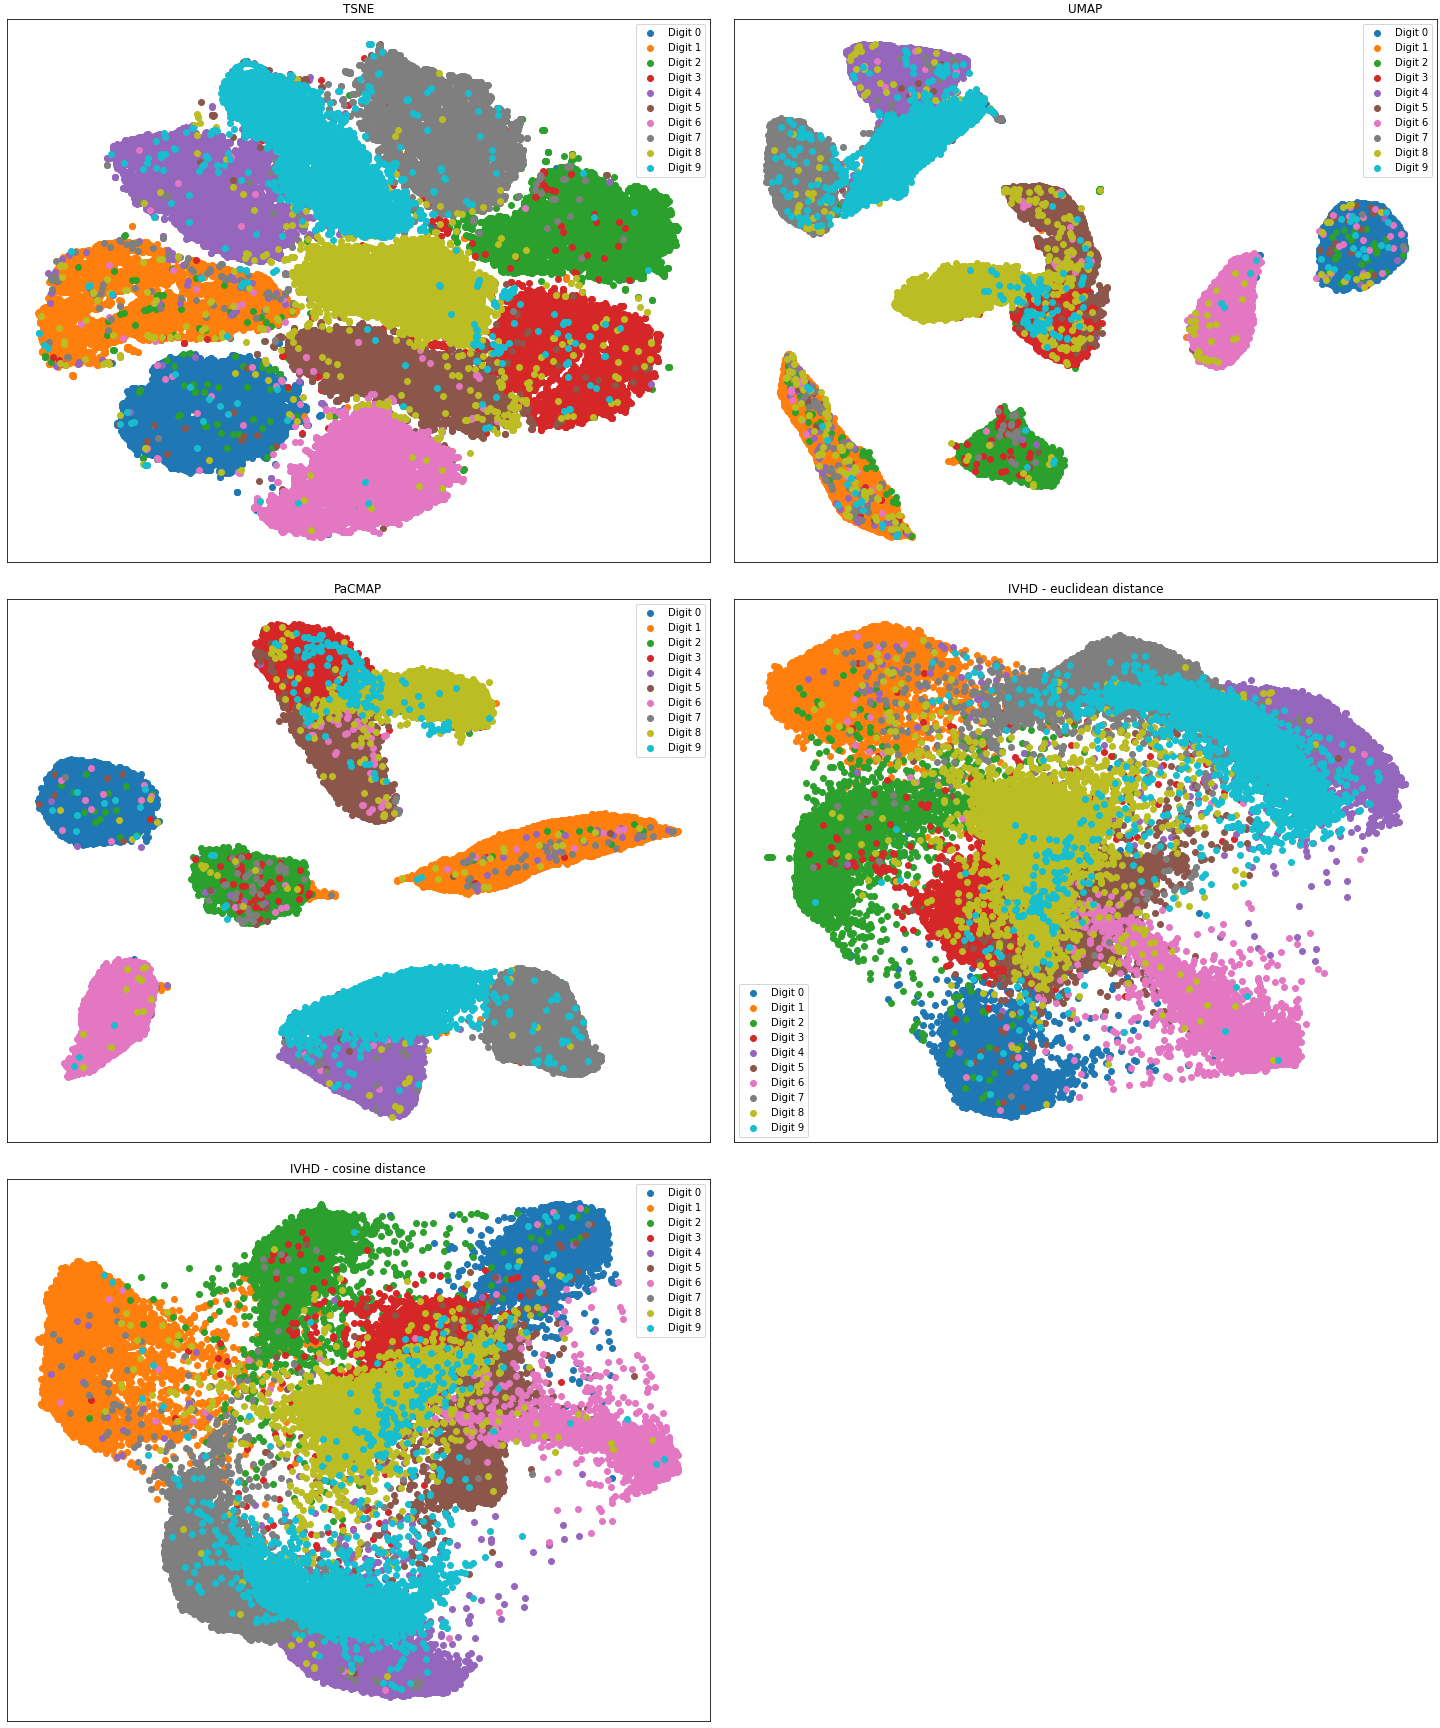
\includegraphics[width=0.65\textwidth]{MNIST/MNIST-collective-visualizations.png}
    \caption{MNIST visualizations using t-SNE, UMAP, PaCMAP and IVHD.}
    \label{fig:mnist_visualization}
\end{figure}
\clearpage
MNIST dataset contains handwritten digits, so we have good intuition how this separation should look like. The default parameterization was used for t-SNE, UMAP and PaCMAP methods. In the case of IVHD, the parameters were set as follows: number of nearest neighbors - 3, number of random neighbors - 2, number of iterations - 5000, rest were set by default. As it can be seen in Figure \ref{fig:mnist_visualization}, good local separation has been achieved for each method. UMAP and PaCMAP methods reflect global separation best. We can tell that there are two three-elements clusters: first includes digits 3, 5 and 8, second includes digits 4, 7, 9. And the rest of the numbers are far from the rest. It coincides with what our intuition would tell us. However, in addition to visual analysis, it is necessary to use metrics to efficiently assess the quality of each embedding.

\subsubsection{Distance matrix-based metric}
\begin{table}[h]
\centering
\caption{Distance matrix-based metric. \\ Results for MNIST embeddings using t-SNE, UMAP, ISOMAP and IVHD.}
\begin{tabular}{|c|c|l|l|l|}
\hline
\textbf{t-SNE} & \textbf{UMAP} & \textbf{PaCMAP}            & \textbf{IVHD euclidean}    & \textbf{IVHD cosine}       \\ \hline
0.346          & 0.168         & \multicolumn{1}{c|}{0.230} & \multicolumn{1}{c|}{0.250} & \multicolumn{1}{c|}{0.206} \\ \hline
\end{tabular}
\end{table}

\subsubsection{Distance matrix-based metric with KMeans optimization}
\begin{table}[h]
\centering
\caption{Distance matrix-based metric with KMeans optimization. \\ Results for 20 News Groups embeddings using t-SNE, UMAP, ISOMAP and IVHD.}
\begin{tabular}{|c|c|l|l|l|}
\hline
\textbf{t-SNE} & \textbf{UMAP} & \textbf{PaCMAP}            & \textbf{IVHD euclidean}    & \textbf{IVHD cosine}       \\ \hline
0.331          & 0.203         & \multicolumn{1}{c|}{0.212} & \multicolumn{1}{c|}{0.241} & \multicolumn{1}{c|}{0.221} \\ \hline
\end{tabular}
\end{table}
Distance matrix-based metric and its optimized version in terms of the execution time return similar results. However, the non-approximation one may be considered more reliable. It is worth recalling that this metric is the quotient of the average distances of points belonging to the same class and inter-class ones. Generally, if the mean distances between points with the same labels decrease, the resulting clusters are tighter and more compact. Furthermore, the value of the metric decreases as the average distances between classes increase, and thus the quality of global separation gets better. Therefore, UMAP yielded the most distinguished clusters. PaCMAP and IVHD turned out to be not much worse. Distance matrix-based metric indicated t-SNE as the worst in terms of the considered criterion. 

\clearpage
\subsubsection{DR quality and KNN gain}
\begin{figure}[h]
\centering
\begin{subfigure}{.5\textwidth}
  \centering
  \includegraphics[width=\linewidth]{MNIST/MNIST-DR-quality.png}
  \label{fig:sub1}
\end{subfigure}%
\begin{subfigure}{.5\textwidth}
  \centering
  \includegraphics[width=\linewidth]{MNIST/MNIST-KNN-gain.png}
  \label{fig:sub2}
\end{subfigure}
\caption{DR quality and KNN gain for MNIST}
\label{fig:test}
\end{figure}
Referring to the DR quality plot, t-SNE provides the highest quality of local separation (up to neighborhood size equal to $10^2$). In the next part of the chart, the dominance of the PaCMAP and UMAP occurs. Furthermore, for the bigger neighborhood size, t-SNE returns worse results than the other dimensionality reduction techniques. Finally, strengthening the analysis with the KNN gain chart, UMAP and PaCMAP performed best.

\clearpage
\subsubsection{Co-ranking matrix}
\begin{figure}[h]
    \centering
    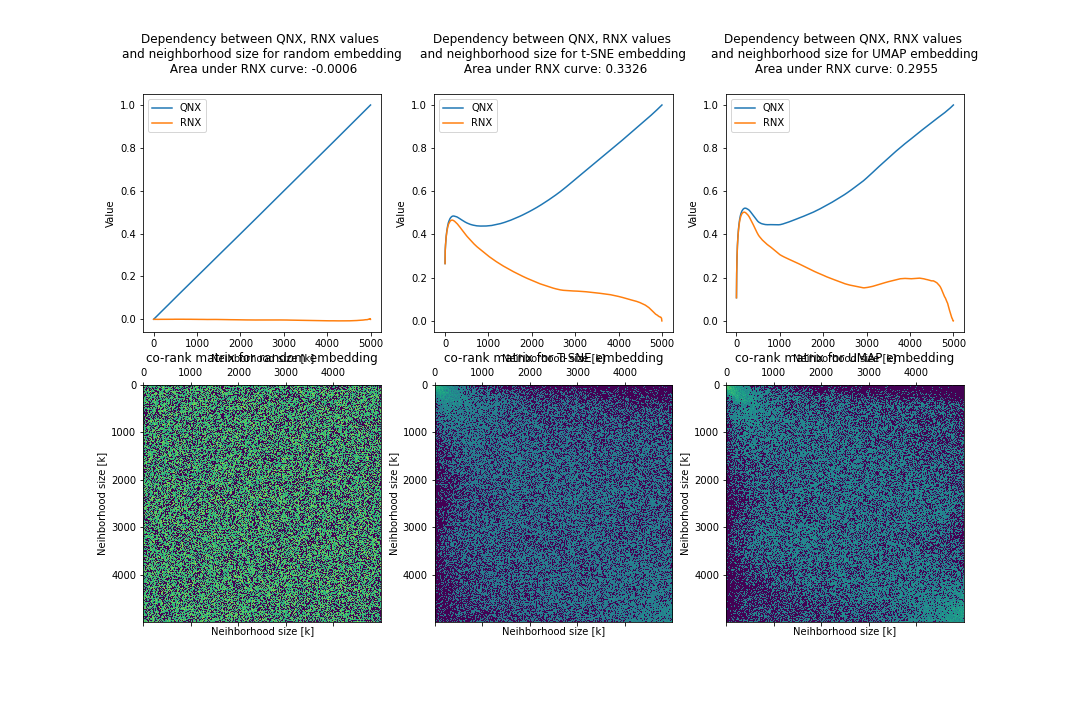
\includegraphics[width=0.95\textwidth]{MNIST/MNIST-co-rank-matrix-part-1.png}
    \caption{Co-ranking matrix-based metrics. \\ Results for MNIST embeddings using random embedding, t-SNE and UMAP.}
\end{figure}
Random embedding pretends the most inaccurate of possible mappings, where the co-ranking matrix visualization looks like complete noise. For real data embedding techniques, it is possible to observe a green cone created, indicating that the mapping to the low-dimensional space is not accidental. Since RNX is a scaled version of QNX, and the area under the RNX curve returns the exact numerical value, it can determine the process of analyzing the accuracy of dimension reduction techniques using this metric. Additionally, for each of the representations, the QNX curve converges to the value 1. It is natural because assuming that P indicates the number of the nearest neighbors and there are P samples in the original dimensionality and reduced one, computations qualify each sample as a neighbor.

\clearpage
\begin{figure}[h]
    \centering
    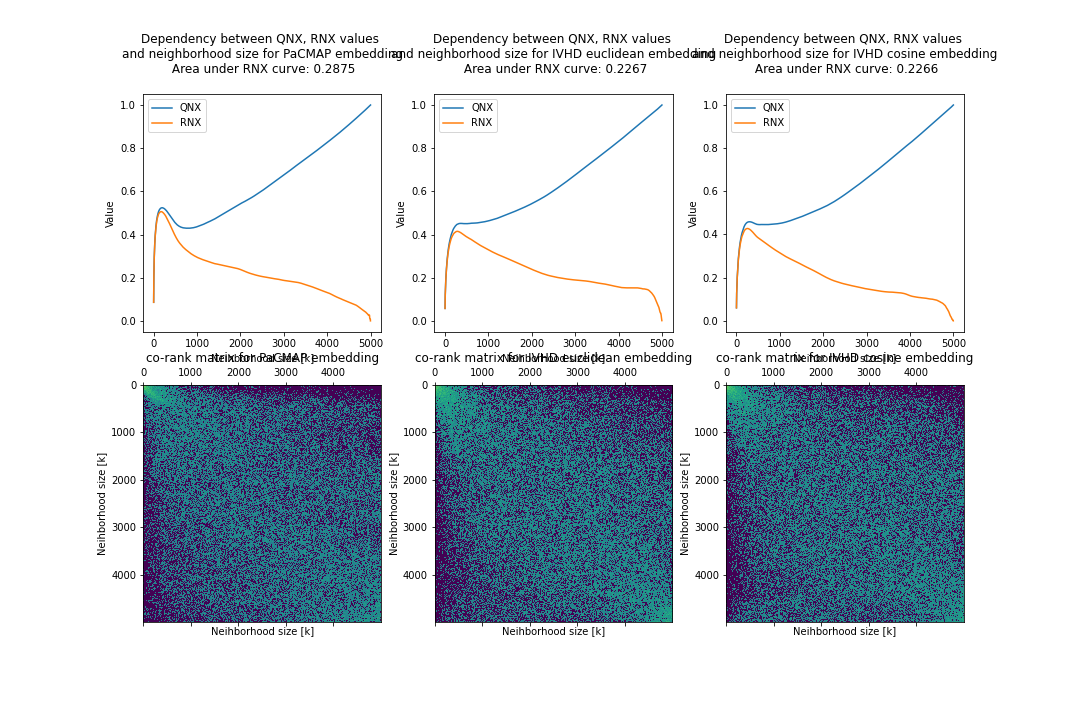
\includegraphics[width=0.95\textwidth]{MNIST/MNIST-co-rank-matrix-part-2.png}
    \caption{Co-ranking matrix-based metrics. \\ Results for MNIST embeddings using PaCMAP and IVHD.}
\end{figure}
The largest area under the RNX curve is for t-SNE, which means that t-SNE achieves the best results for the local neighborhood (small K size).

\clearpage
\subsubsection{Shepard diagrams}

\begin{figure}[h]
    \centering
    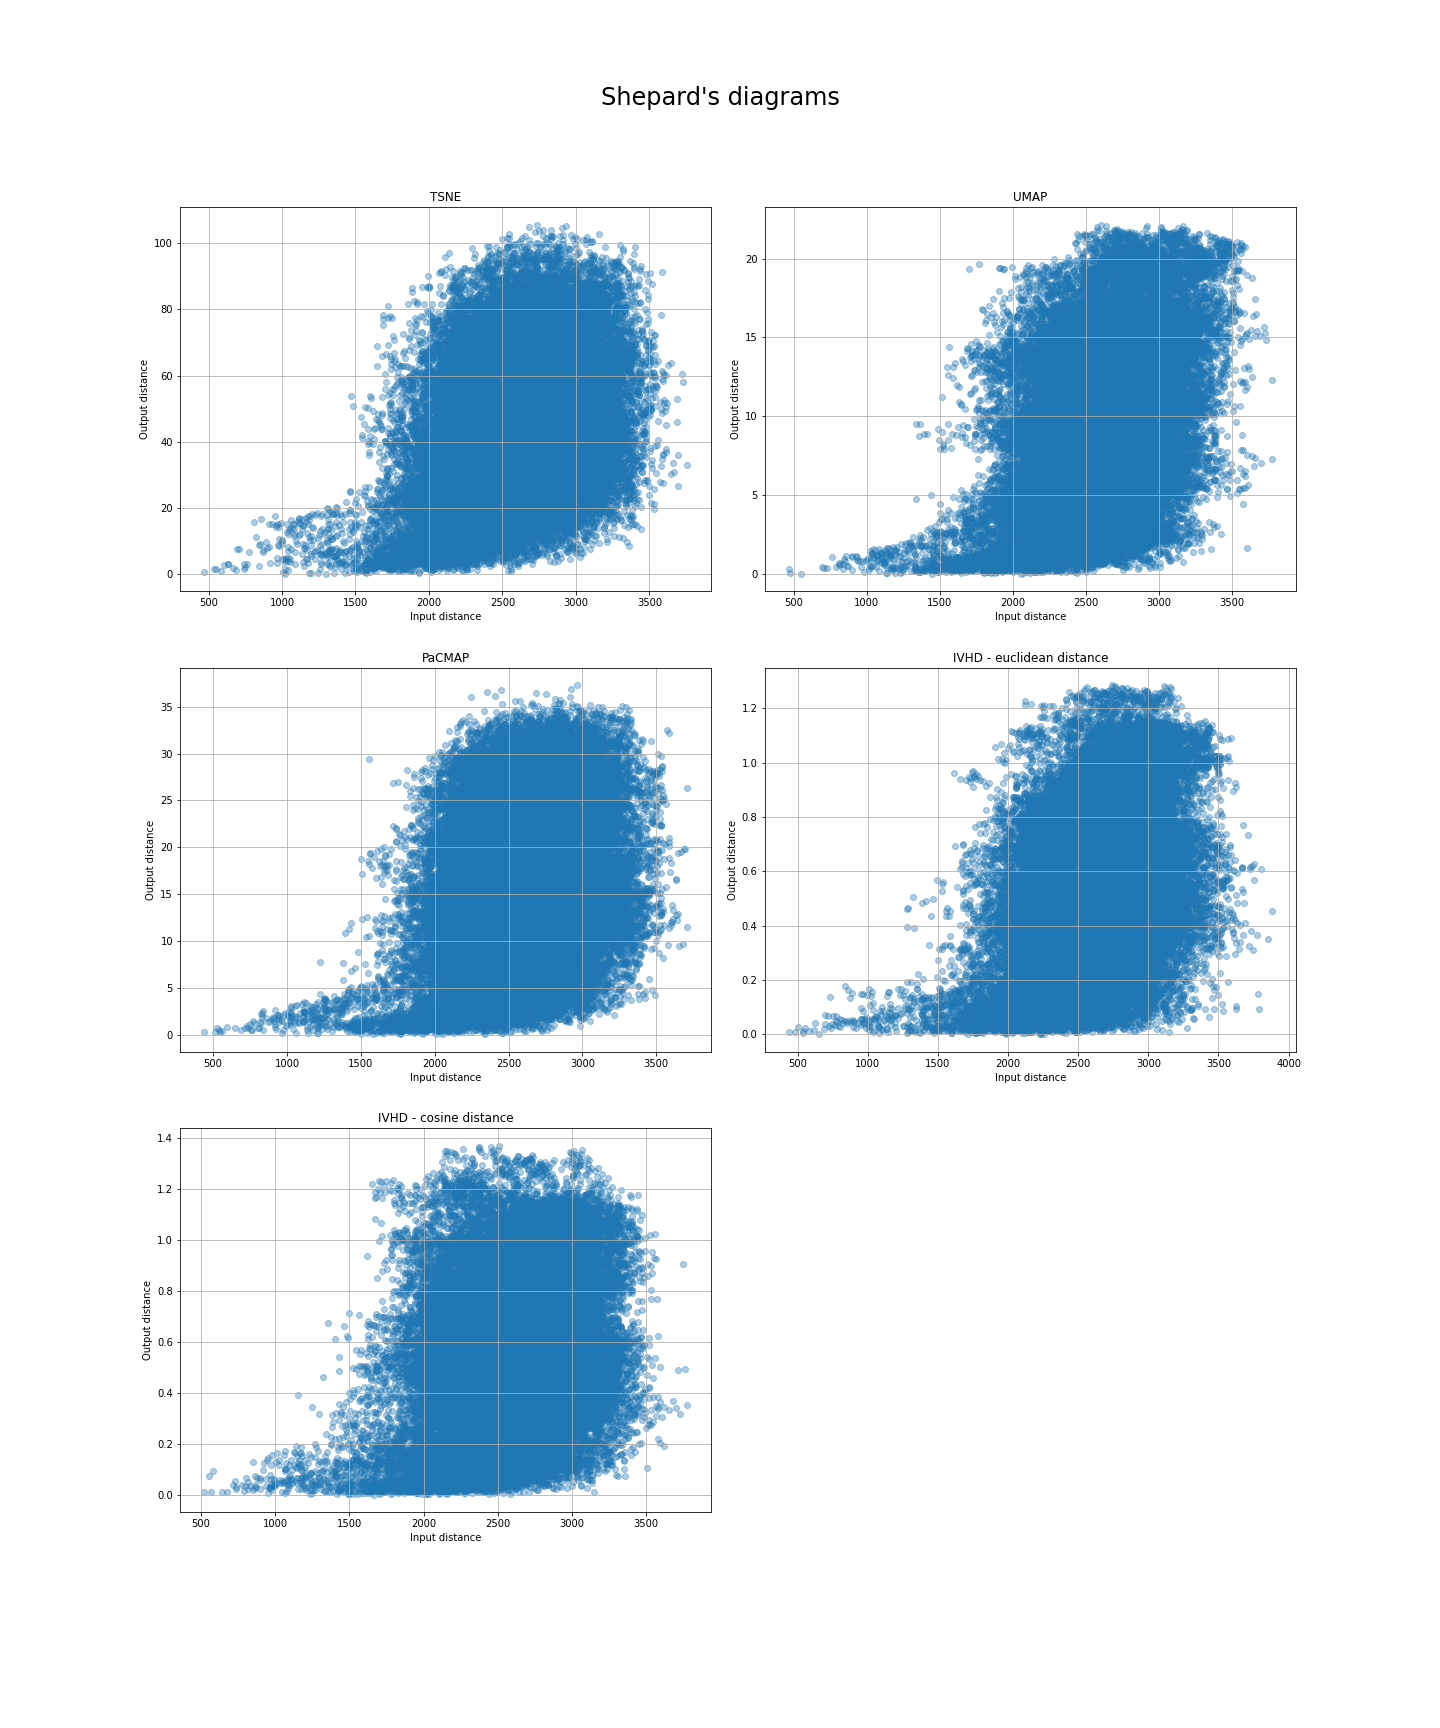
\includegraphics[width=0.8\textwidth]{MNIST/MNIST-shepard-diagrams.png}
    \caption{Shepard diagrams of MNIST embeddings using t-SNE, UMAP, PaCMAP and IVHD.}
\end{figure}
Ideally, the points in the Sheppard diagram should be on a straight line which would mean that the distances in the reduced dimensionality are perfectly rescaled values from the original space. We can see that the points are rather heavily scattered around than spread along the straight line. For PaCMAP and UMAP we can notice that the group of points is the most compact and there are the fewest points far away from the straight line.

\clearpage
\subsubsection{Trustworthiness}
\begin{table}[h]
\centering
\caption{Trustworthiness with euclidean metric for pairwise distances. \\
Results for MNIST embeddings using t-SNE, UMAP, ISOMAP and IVHD.}
\begin{tabular}{|c|c|c|c|c|c|}
\hline
\textbf{K} & \textbf{t-SNE} & \textbf{UMAP} & \multicolumn{1}{l|}{\textbf{PaCMAP}} & \multicolumn{1}{l|}{\textbf{IVHD euclidean}} & \multicolumn{1}{l|}{\textbf{IVHD cosine}} \\ \hline
5          & 0.980          & 0.959         & 0.957                                & 0.887                                        & 0.896                                     \\ \hline
15         & 0.970          & 0.955         & 0.956                                & 0.884                                        & 0.893                                     \\ \hline
50         & 0.948          & 0.947         & 0.946                                & 0.877                                        & 0.889                                     \\ \hline
100        & 0.927          & 0.936         & 0.936                                & 0.870                                        & 0.883                                     \\ \hline
150        & 0.908          & 0.924         & 0.924                                & 0.863                                        & 0.875                                     \\ \hline
\end{tabular}
\end{table}
The high values of the trustworthiness metric obtained for all embedding techniques indicate that each method coped relatively well with local separation. This conclusion coincides with the results of visualizations, where each class creates a distinctive cluster. Consistency in good results should be taken into account, which indicates that UMAP and PaCMAP methods were the best at maintaining local relationships between points.

\begin{table}[h]
\centering
\caption{Trustworthiness with cosine metric for pairwise distances. \\
Results for MNIST embeddings using t-SNE, UMAP, ISOMAP and IVHD.}
\begin{tabular}{|c|c|c|c|c|c|}
\hline
\textbf{K} & \textbf{t-SNE} & \textbf{UMAP} & \multicolumn{1}{l|}{\textbf{PaCMAP}} & \multicolumn{1}{l|}{\textbf{IVHD euclidean}} & \multicolumn{1}{l|}{\textbf{IVHD cosine}} \\ \hline
5          & 0.984          & 0.969         & 0.967                                & 0.892                                        & 0.910                                     \\ \hline
15         & 0.975          & 0.967         & 0.965                                & 0.890                                        & 0.909                                     \\ \hline
50         & 0.959          & 0.961         & 0.960                                & 0.885                                        & 0.905                                     \\ \hline
100        & 0.941          & 0.953         & 0.953                                & 0.879                                        & 0.900                                     \\ \hline
150        & 0.924          & 0.943         & 0.944                                & 0.873                                        & 0.892                                     \\ \hline
\end{tabular}
\end{table}

\subsubsection{Spearman correlation-based metric}
\begin{table}[h]
\centering
\caption{Spearman correlation-based metric. \\ Results for MNIST embeddings using t-SNE, UMAP, PaCMAP and IVHD.}
\begin{tabular}{|c|c|l|l|l|}
\hline
\textbf{t-SNE} & \textbf{UMAP} & \textbf{PaCMAP}            & \textbf{IVHD euclidean}    & \textbf{IVHD cosine}       \\ \hline
0.666          & 0.683         & \multicolumn{1}{c|}{0.700} & \multicolumn{1}{c|}{0.545} & \multicolumn{1}{c|}{0.575} \\ \hline
\end{tabular}
\end{table}
The metric based on Spearman's correlation places t-SNE, UMAP, and PaCMAP on the podium, but the last of them turned out to be the most faithful in maintaining the correlation between the distances in both dimensions.

%%%%%%%%%%%%%%%%%%%%%%%%%%%%%%%%%%%%%%%%%%%%%%%%%%%%%%%%%%%%%%%%%%%%%%%%%%%%%%%%%%%%
\clearpage
\subsection{20 News Groups}
In this subsection, analysis of 20 News Groups dataset is presented. A code which was used to get these results can be found in our repository\cite{github-20ng}.
\subsubsection{Visualizations}
\begin{figure}[h]
    \centering
    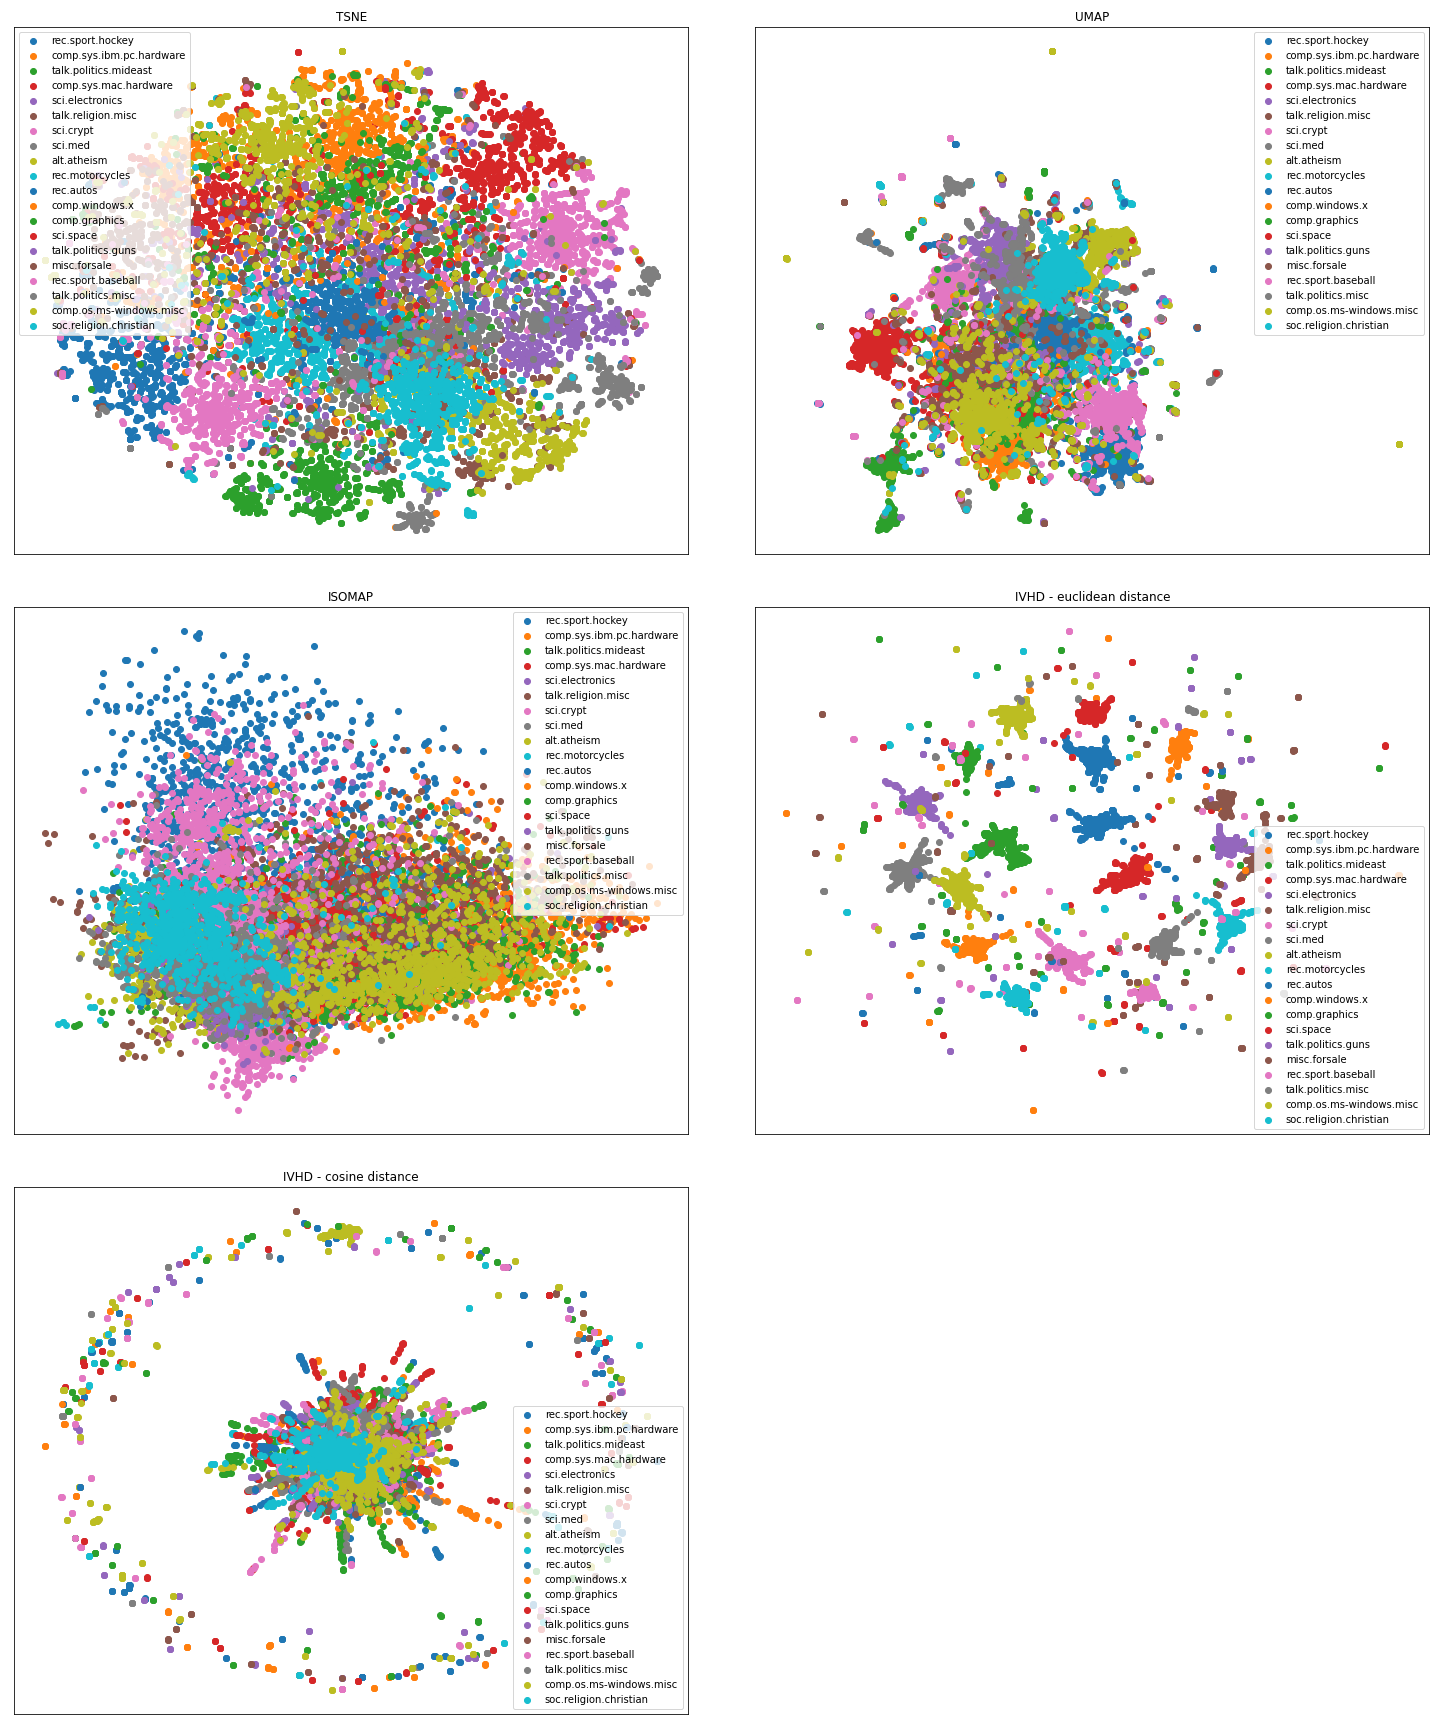
\includegraphics[width=0.80\textwidth]{20 NG/20NG-collective-visualizations.png}
    \caption{20 News Groups visualizations using t-SNE, UMAP, ISOMAP and IVHD.}
    \label{fig:20ng_vis}
\end{figure}

\clearpage
In case of this dataset in t-SNE method perplexity parameter was set to 15, in other method default parametrization was used. IVHD with cosine distance metric gave worst results, but with Euclidean distance metric obtained results were very good separated globally and locally. For different datasets, different distance metrics give better results. As we can see in Figure \ref{fig:20ng_vis} every method gives good local separation. Global separation is only easy to see in IVHD with Euclidean distance metric, in other methods this separation is a bit blurry. Also, IVHD creates some noise in embedding.

\subsubsection{Distance matrix-based metric}
\begin{table}[h]
\centering
\caption{Distance matrix-based metric. \\ Results for 20 News Groups embeddings using t-SNE, UMAP, ISOMAP and IVHD.}
\begin{tabular}{|c|c|l|l|l|}
\hline
\textbf{t-SNE} & \textbf{UMAP} & \textbf{ISOMAP}            & \textbf{IVHD euclidean}    & \textbf{IVHD cosine}       \\ \hline
0.574          & 0.639         & \multicolumn{1}{c|}{0.637} & \multicolumn{1}{c|}{0.174} & \multicolumn{1}{c|}{0.314} \\ \hline
\end{tabular}
\end{table}

\subsubsection{Distance matrix-based metric with KMeans optimization}
\begin{table}[h]
\centering
\caption{Distance matrix-based metric with KMeans optimization. \\ Results for 20 News Groups embeddings using t-SNE, UMAP, ISOMAP and IVHD.}
\begin{tabular}{|c|c|l|l|l|}
\hline
\textbf{t-SNE} & \textbf{UMAP} & \textbf{ISOMAP}            & \textbf{IVHD euclidean}    & \textbf{IVHD cosine}       \\ \hline
0.547          & 0.556         & \multicolumn{1}{c|}{0.582} & \multicolumn{1}{c|}{0.182} & \multicolumn{1}{c|}{0.291} \\ \hline
\end{tabular}
\end{table}
Distance matrix-based metric indicated IVHD euclidean as unrivaled in terms of the quality of the created clusters for samples from the same classes. According to this metric, it is precisely after the application of IVHD cosine that the most compact clusters can be obtained.

\clearpage
\subsubsection{DR quality and KNN gain}
\begin{figure}[h]
\centering
\begin{subfigure}{.5\textwidth}
  \centering
  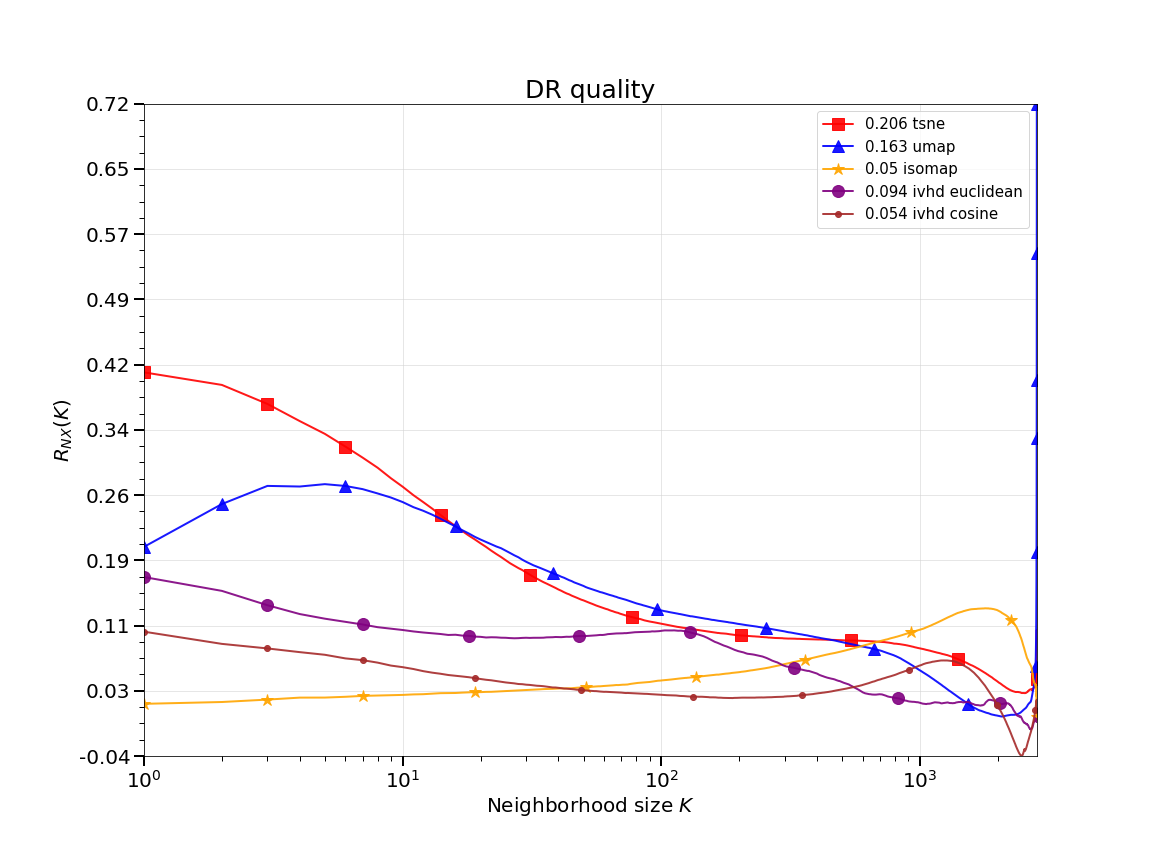
\includegraphics[width=\linewidth]{20 NG/20NG-dr-quality.png}
  \label{fig:sub1}
\end{subfigure}%
\begin{subfigure}{.5\textwidth}
  \centering
  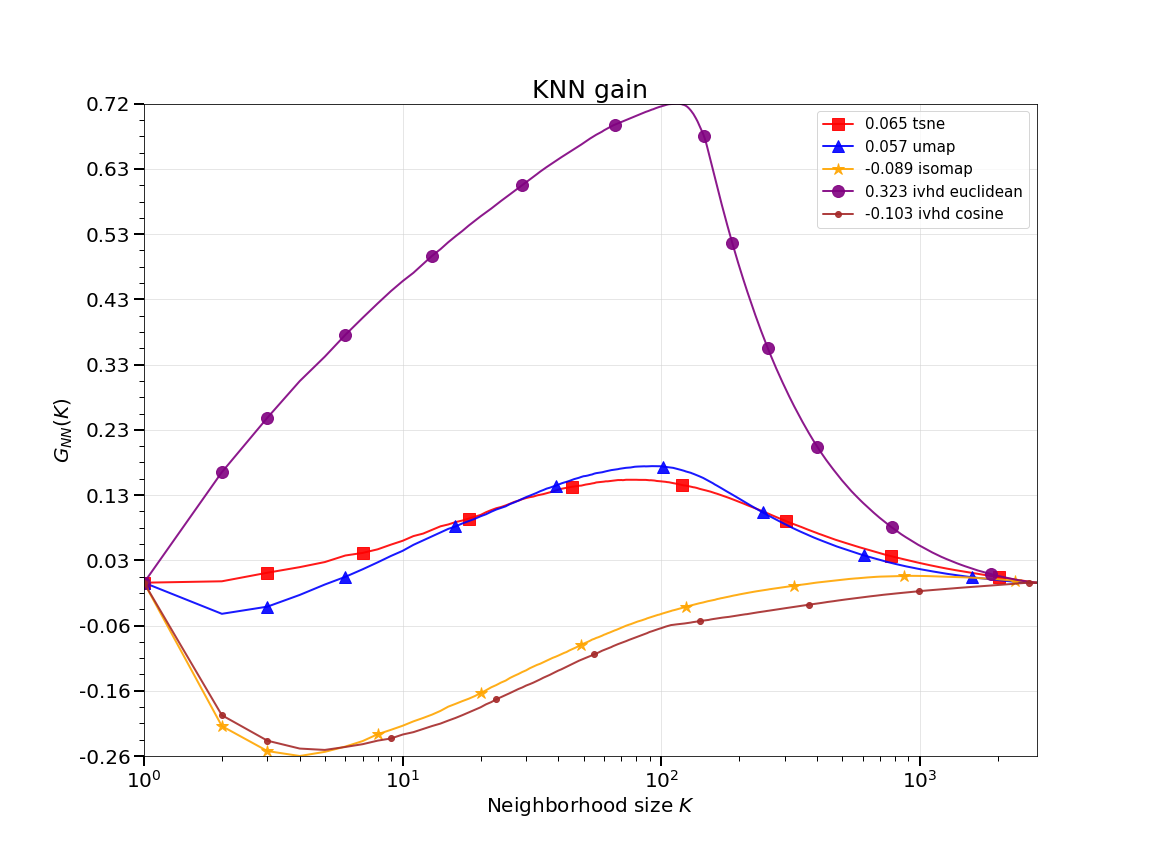
\includegraphics[width=\linewidth]{20 NG/20NG-knn-gain.png}
  \label{fig:sub2}
\end{subfigure}
\caption{DR quality and KNN gain for 20 News Groups}
\label{fig:test}
\end{figure}
The KNN gain graph clearly illustrates the contrast between IVHD euclidean and IVHD cosine. The first variant allows to achieve by far the best separation - the resulting clusters are separated from the others. On the other hand, the IVHD cosine failed at outlining dependencies from the original space. Again, t-SNE proved to be the best for local separation. However, when confronting the results jointly with visualizations and both metric charts, IVHD euclidean indisputably brings the best result of global separation.

\clearpage
\subsubsection{Co-ranking matrix}
\begin{figure}[h]
    \centering
    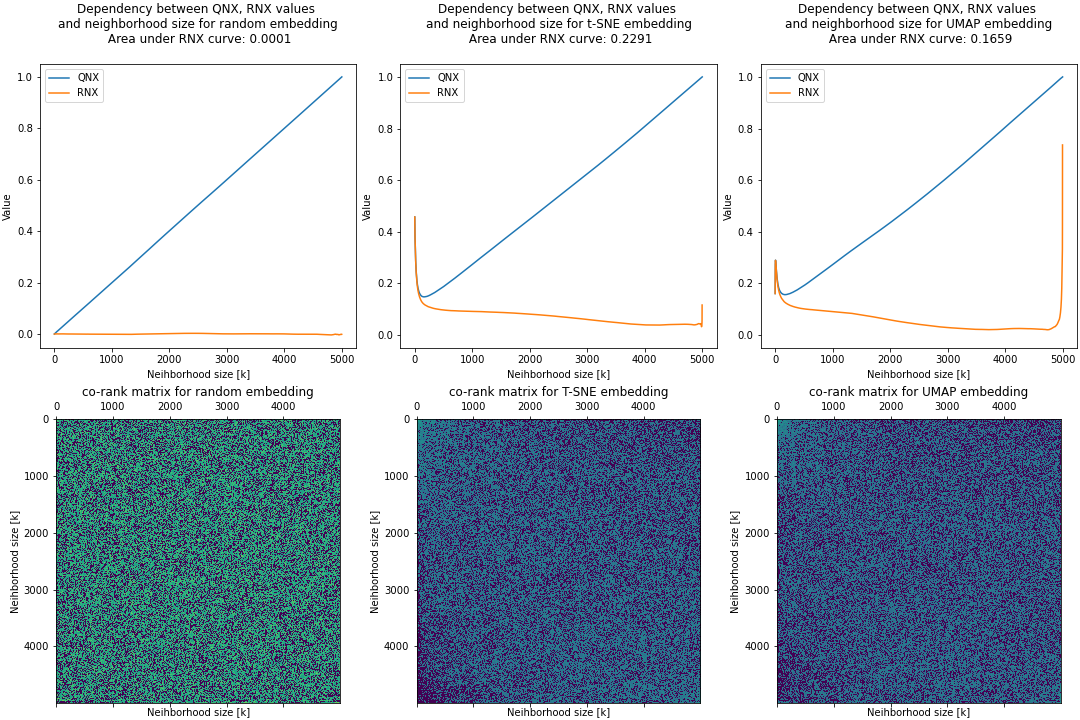
\includegraphics[width=0.95\textwidth]{20 NG/20NG-co-rank-matrix-part-1.png}
    \caption{Co-ranking matrix-based metrics. \\ Results for 20 News Groups embeddings using random embedding, t-SNE and UMAP.}
\end{figure}

\clearpage
\begin{figure}[h]
    \centering
    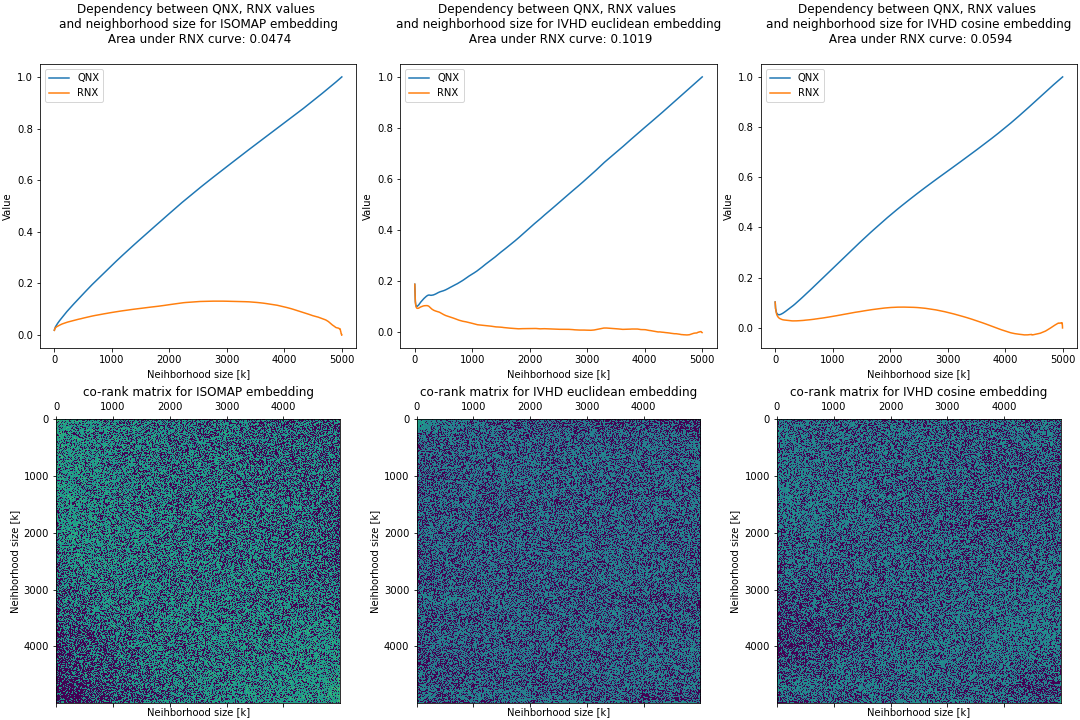
\includegraphics[width=0.95\textwidth]{20 NG/20NG-co-rank-matrix-part-2.png}
    \caption{Co-ranking matrix-based metrics. \\ Results for 20 News Groups embeddings using ISOMAP and IVHD.}
\end{figure}
The results indicate a significant challenge for data embedding techniques to preserve the local neighborhood in the reduced dimensionality. However, the best results are for t-SNE (the initial most steep trend of the RNX curve) and simultaneously the highest value of the area under the RNX curve.

\clearpage
\subsubsection{Shepard diagrams}
\begin{figure}[h]
    \centering
    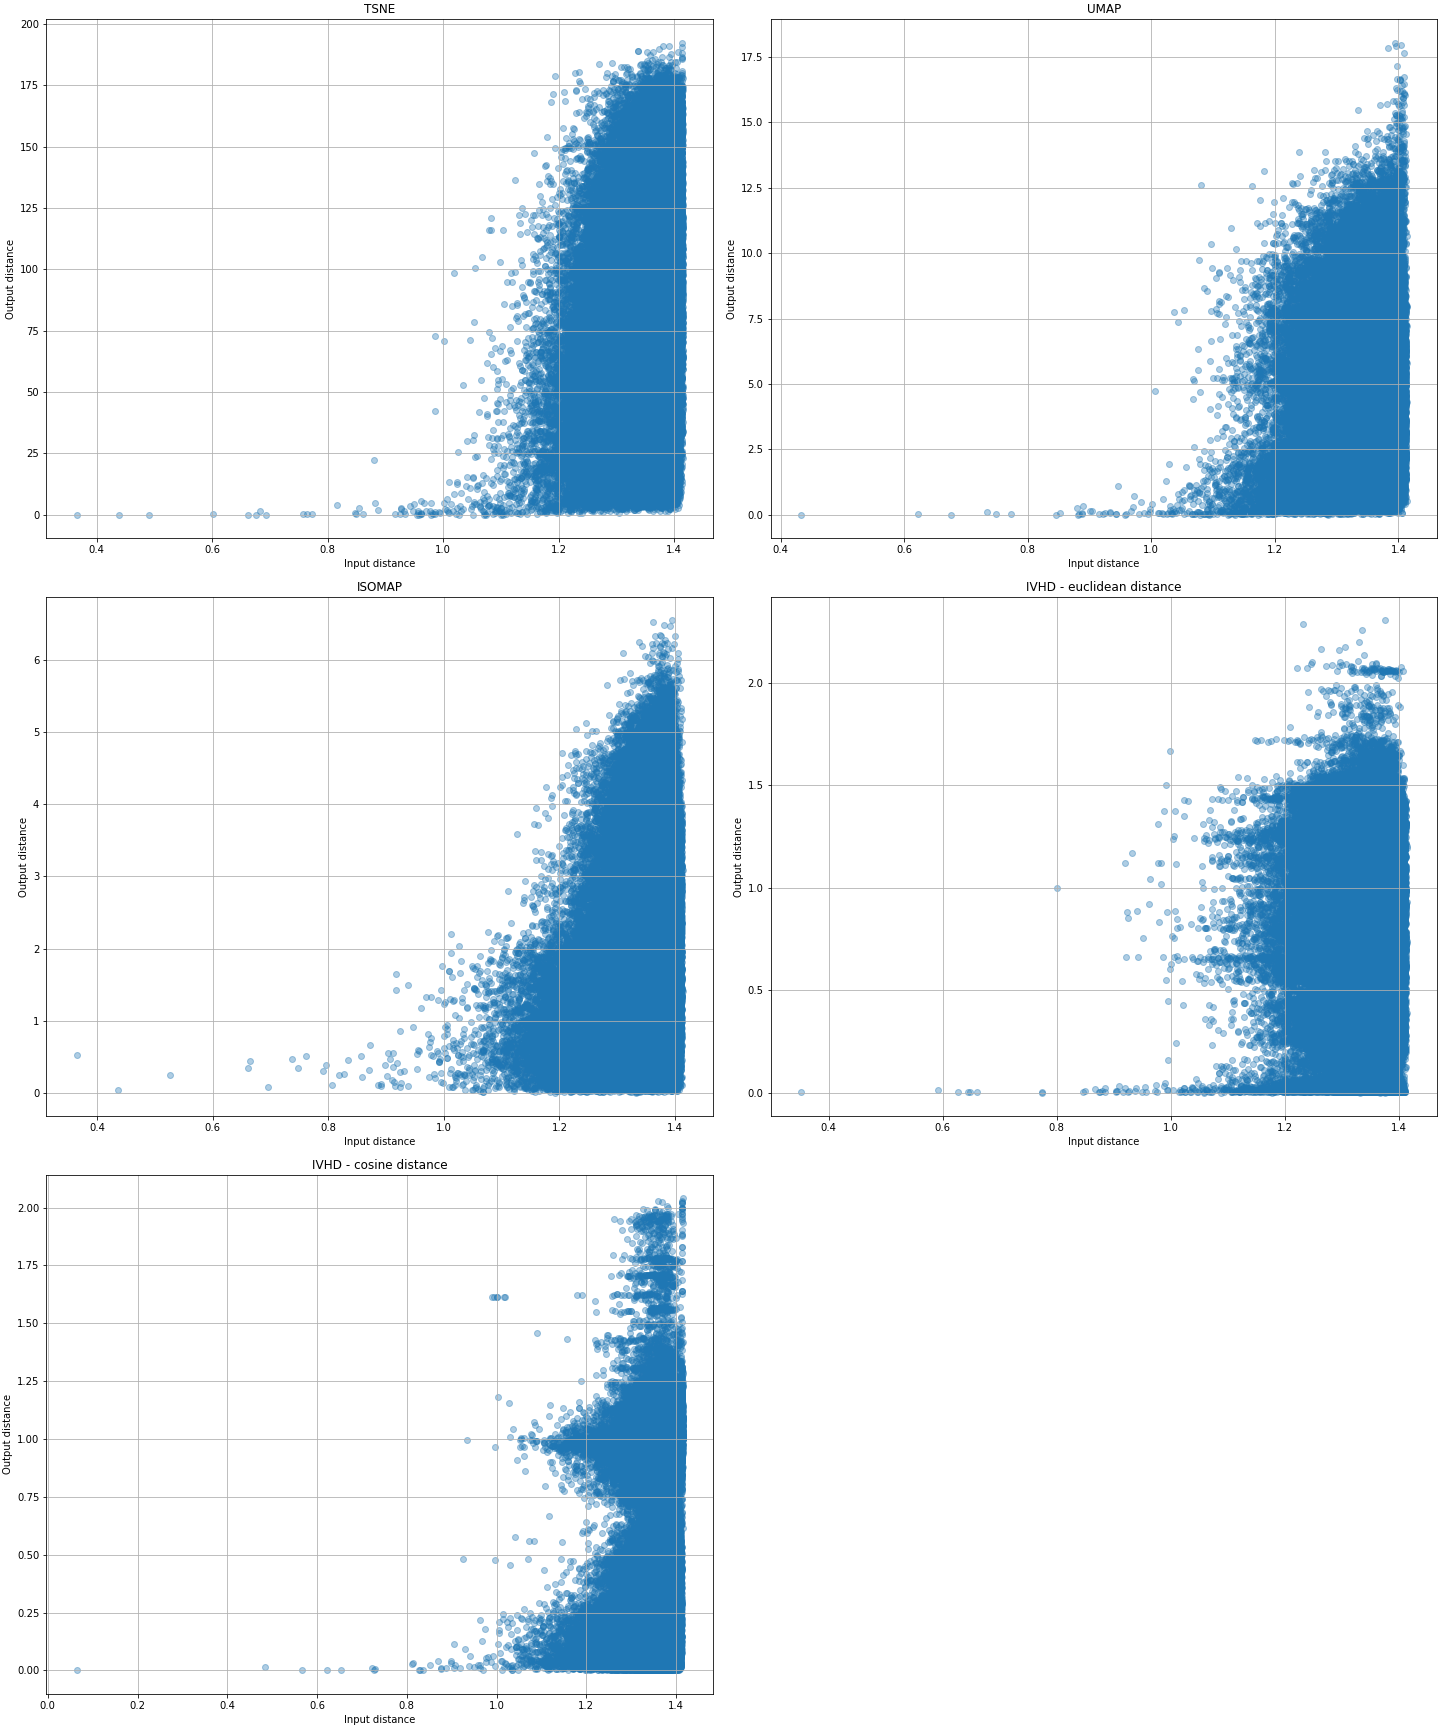
\includegraphics[width=0.8\textwidth]{20 NG/20NG-shepard-diagrams.png}
    \caption{Shepard diagrams of 20 News Groups embeddings using t-SNE, UMAP, ISOMAP and IVHD.}
\end{figure}
The Shepard diagram for all techniques except IVHD has the most concise and least jagged form. In summarizing, all scatter plots are far from ideal. Finally, in the case of IVHD euclidean, it is possible to observe a lot of points detached from the group, which may indicate that, apart from the distinguished clusters, many points identifies as noise.

\clearpage
\subsubsection{Trustworthiness}
\begin{table}[h]
\centering
\caption{Trustworthiness with euclidean metric for pairwise distances. \\
Results for 20 News Groups embeddings using t-SNE, UMAP, ISOMAP and IVHD.}
\begin{tabular}{|c|c|c|c|c|c|}
\hline
\textbf{K} & \textbf{t-SNE} & \textbf{UMAP} & \multicolumn{1}{l|}{\textbf{ISOMAP}} & \multicolumn{1}{l|}{\textbf{IVHD euclidean}} & \multicolumn{1}{l|}{\textbf{IVHD cosine}} \\ \hline
5          & 0.880          & 0.838         & 0.574                                & 0.704                                        & 0.583                                     \\ \hline
15         & 0.784          & 0.775         & 0.570                                & 0.670                                        & 0.559                                     \\ \hline
50         & 0.678          & 0.686         & 0.571                                & 0.648                                        & 0.541                                     \\ \hline
100        & 0.638          & 0.650         & 0.573                                & 0.643                                        & 0.537                                     \\ \hline
150        & 0.662          & 0.634         & 0.575                                & 0.636                                        & 0.536                                     \\ \hline
\end{tabular}
\end{table}
Both for euclidean and cosine distances, trustworthiness yielded around identical values. For a small neighborhood, the t-SNE method obtained the best results, but the farther away, the gains resulting from IVHD euclidean can be observed.

\begin{table}[h]
\centering
\caption{Trustworthiness with cosine metric for pairwise distances. \\
Results for 20 News Groups embeddings using t-SNE, UMAP, ISOMAP and IVHD.}
\begin{tabular}{|c|c|c|c|c|c|}
\hline
\textbf{K} & \textbf{t-SNE} & \textbf{UMAP} & \multicolumn{1}{l|}{\textbf{ISOMAP}} & \multicolumn{1}{l|}{\textbf{IVHD euclidean}} & \multicolumn{1}{l|}{\textbf{IVHD cosine}} \\ \hline
5          & 0.880          & 0.838         & 0.574                                & 0.704                                        & 0.583                                     \\ \hline
15         & 0.784          & 0.775         & 0.570                                & 0.670                                        & 0.559                                     \\ \hline
50         & 0.678          & 0.686         & 0.571                                & 0.648                                        & 0.541                                     \\ \hline
100        & 0.638          & 0.650         & 0.573                                & 0.643                                        & 0.537                                     \\ \hline
150        & 0.622          & 0.634         & 0.575                                & 0.636                                        & 0.536                                     \\ \hline
\end{tabular}
\end{table}

\subsubsection{Spearman correlation-based metric}
\begin{table}[h]
\centering
\caption{Spearman correlation-based metric. \\ Results for 20 News Groups embeddings using t-SNE, UMAP, ISOMAP and IVHD.}
\begin{tabular}{|c|c|l|l|l|}
\hline
\textbf{t-SNE} & \textbf{UMAP} & \textbf{ISOMAP}            & \textbf{IVHD euclidean}    & \textbf{IVHD cosine}       \\ \hline
0.259          & 0.286         & \multicolumn{1}{c|}{0.181} & \multicolumn{1}{c|}{0.132} & \multicolumn{1}{c|}{0.112} \\ \hline
\end{tabular}
\end{table}
Relatively low metric values may indicate that the 20 News Groups turned out to be challenging to separate. However, the UMAP and t-SNE retained the strongest correlation between distances in the original space and reduced dimensionality.

%%%%%%%%%%%%%%%%%%%%%%%%%%%%%%%%%%%%%%%%%%%%%%%%%%%%%%%%%%%%%%%%%%%%%%%%%%%%%%%%%%%%%%%%%%%%%%%%%%%%%%%%%%%%%%%%
%%%%%%%%%%%%%%%%%%%%%%%%%%%%%%%%%%%% REUTERS %%%%%%%%%%%%%%%%%%%%%%%%%%%%%%%%%%%%%%%%%%%%%%%%%%%%%%%%%%%%%%%%%%%

\clearpage
\subsection{RCV Reuters}
In this subsection, analysis of RCV Reuters dataset is presented. A code which was used to get these results can be found in our repository\cite{github-reuters}.

\subsubsection{Visualizations}
\begin{figure}[h]
    \centering
    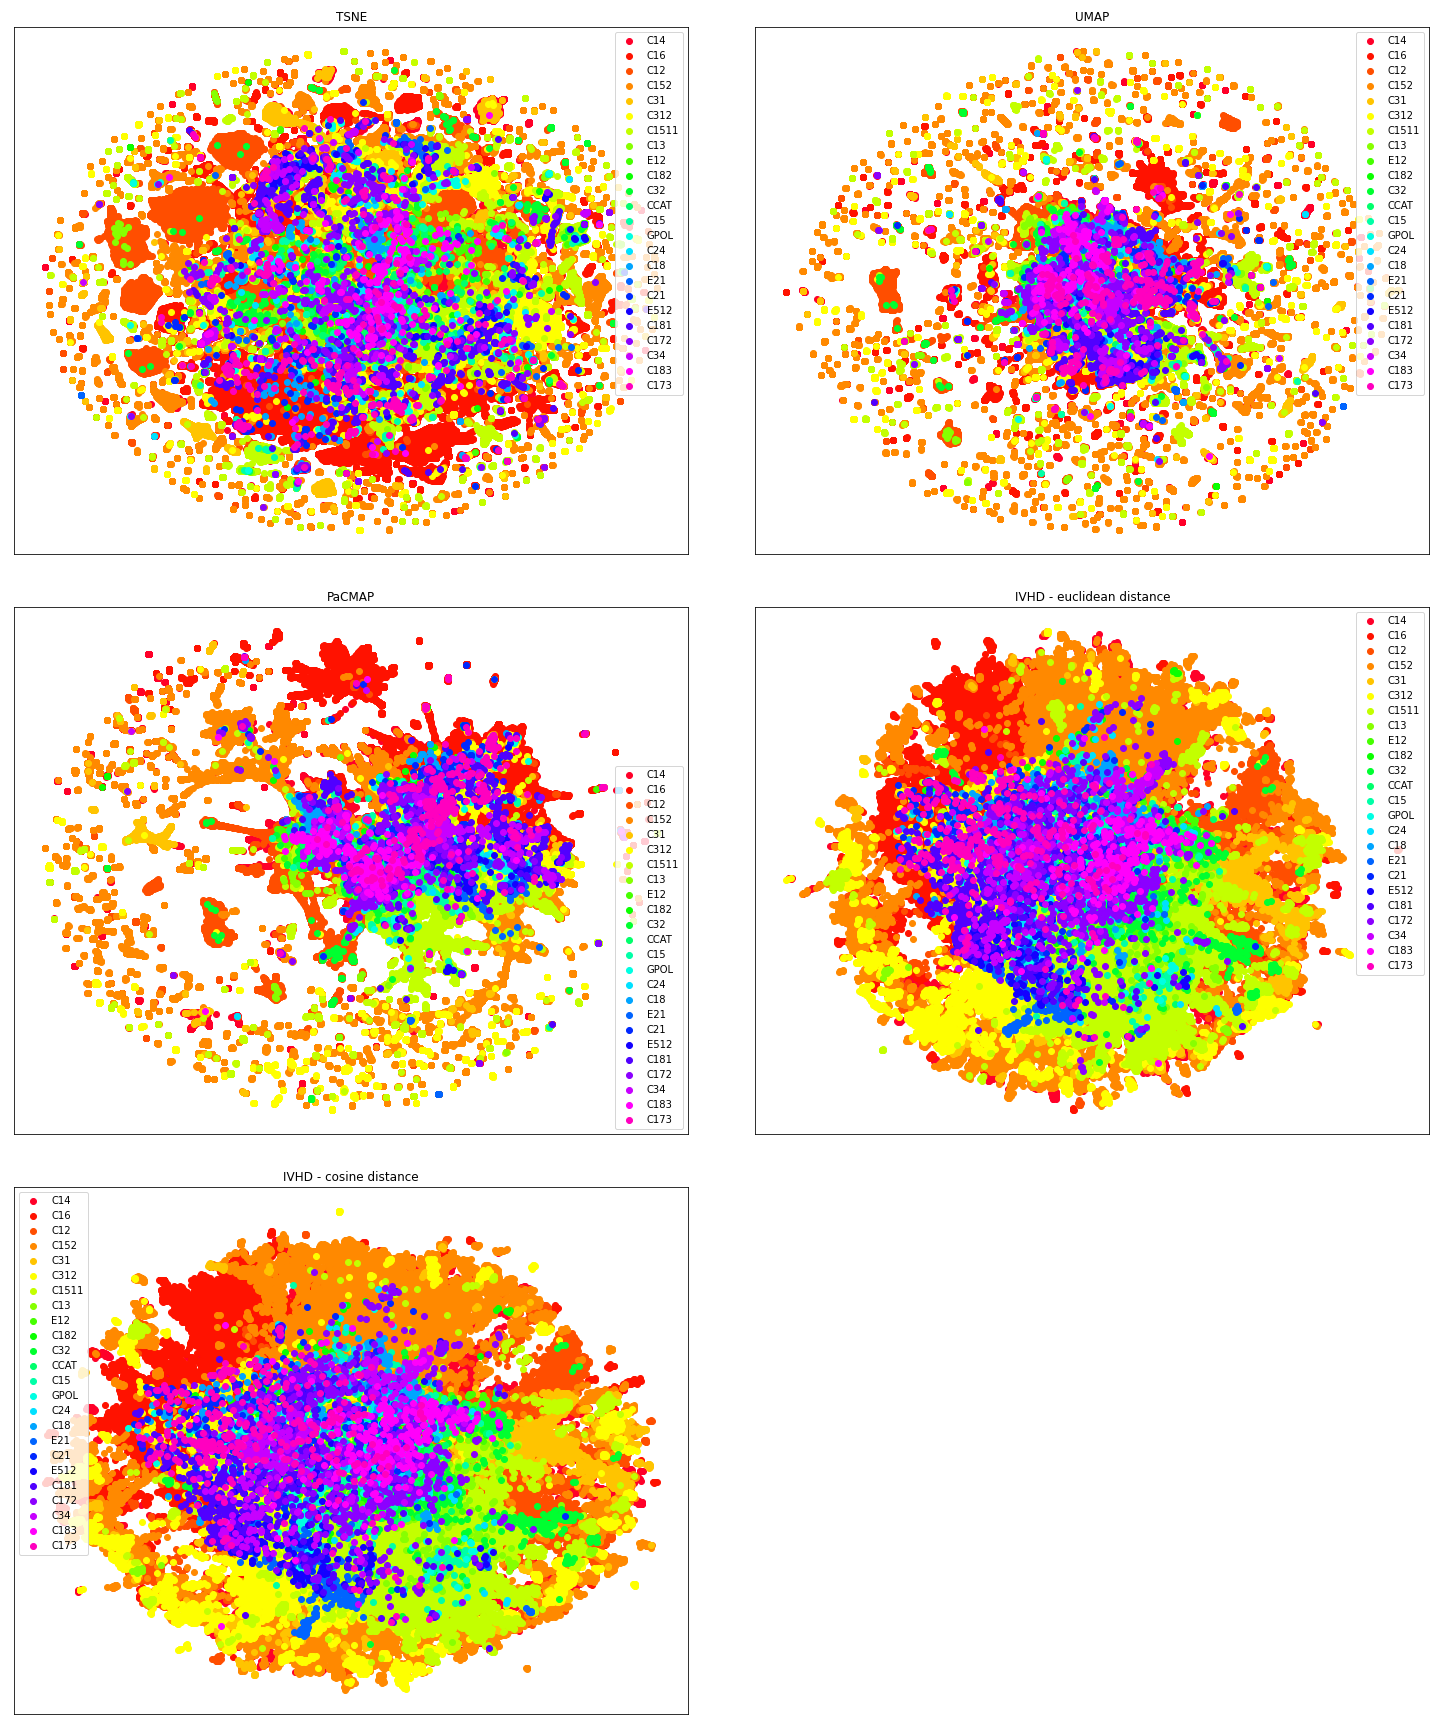
\includegraphics[width=0.80\textwidth]{RCV Reuters/RCV-Reuters-collective-visualizations.png}
    \caption{RCV Reuters visualizations using t-SNE, UMAP, PaCMAP and IVHD.}
    \label{fig:reuters_vis}
\end{figure}
\clearpage

In case of this dataset the following parametrization was used: for t-SNE method perplexity was set to 40, for IVHD number of nearest neighbors was set to 5, number of iterations to 5000 and c to 0.1, other parameters were left default. RCV Reuters is a very complex dataset so as it can be seen in Figure \ref{fig:reuters_vis} presented methods did not reflect the data structure very well. t-SNE, UMAP and PaCMAP methods leave a lot of points alone. Visually, the best local separation is given by IVHD. Neither of the methods reproduced global separation very well.

\subsubsection{Distance matrix-based metric}
\begin{table}[h]
\centering
\caption{Distance matrix-based metric. \\ Results for RCV Reuters embeddings using t-SNE, UMAP, PaCMAP and IVHD.}
\begin{tabular}{|c|c|l|l|l|}
\hline
\textbf{t-SNE} & \textbf{UMAP} & \textbf{PaCMAP}            & \textbf{IVHD euclidean}    & \textbf{IVHD cosine}       \\ \hline
0.804          & 0.650         & \multicolumn{1}{c|}{0.613} & \multicolumn{1}{c|}{0.551} & \multicolumn{1}{c|}{0.548} \\ \hline
\end{tabular}
\end{table}

\subsubsection{Distance matrix-based metric with KMeans optimization}
\begin{table}[h]
\centering
\caption{Distance matrix-based metric with KMeans optimization. \\ Results for RCV Reuters embeddings using t-SNE, UMAP, PaCMAP and IVHD.}
\begin{tabular}{|c|c|l|l|l|}
\hline
\textbf{t-SNE} & \textbf{UMAP} & \textbf{PaCMAP}            & \textbf{IVHD euclidean}    & \textbf{IVHD cosine}       \\ \hline
0.728          & 0.501         & \multicolumn{1}{c|}{0.452} & \multicolumn{1}{c|}{0.503} & \multicolumn{1}{c|}{0.508} \\ \hline
\end{tabular}
\end{table}
The metric based on the distance matrix indicates t-SNE as the one that yields the highest ratio between the mean distances of points in the same class and samples labeled otherly. In fact, in t-SNE, it is hard to distinguish regions where the concentration of samples occurs - it is an even distribution. By citing the value of distance matrix-based metrics without KMeans optimization, IVHD gets the best score.

\clearpage
\subsubsection{DR quality and KNN gain}
\begin{figure}[h]
\centering
\begin{subfigure}{.5\textwidth}
  \centering
  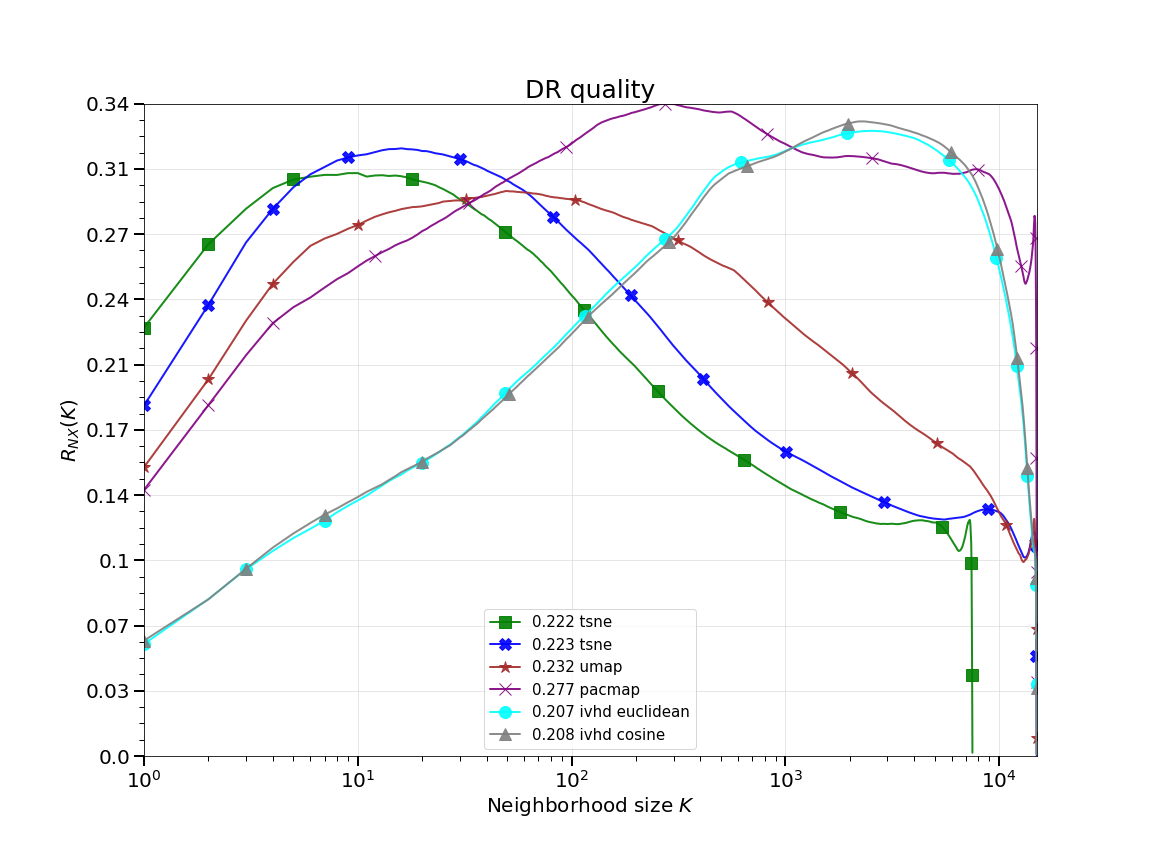
\includegraphics[width=\linewidth]{RCV Reuters/RCV-Reuters-dr-quality.png}
  \label{fig:sub1}
\end{subfigure}%
\begin{subfigure}{.5\textwidth}
  \centering
  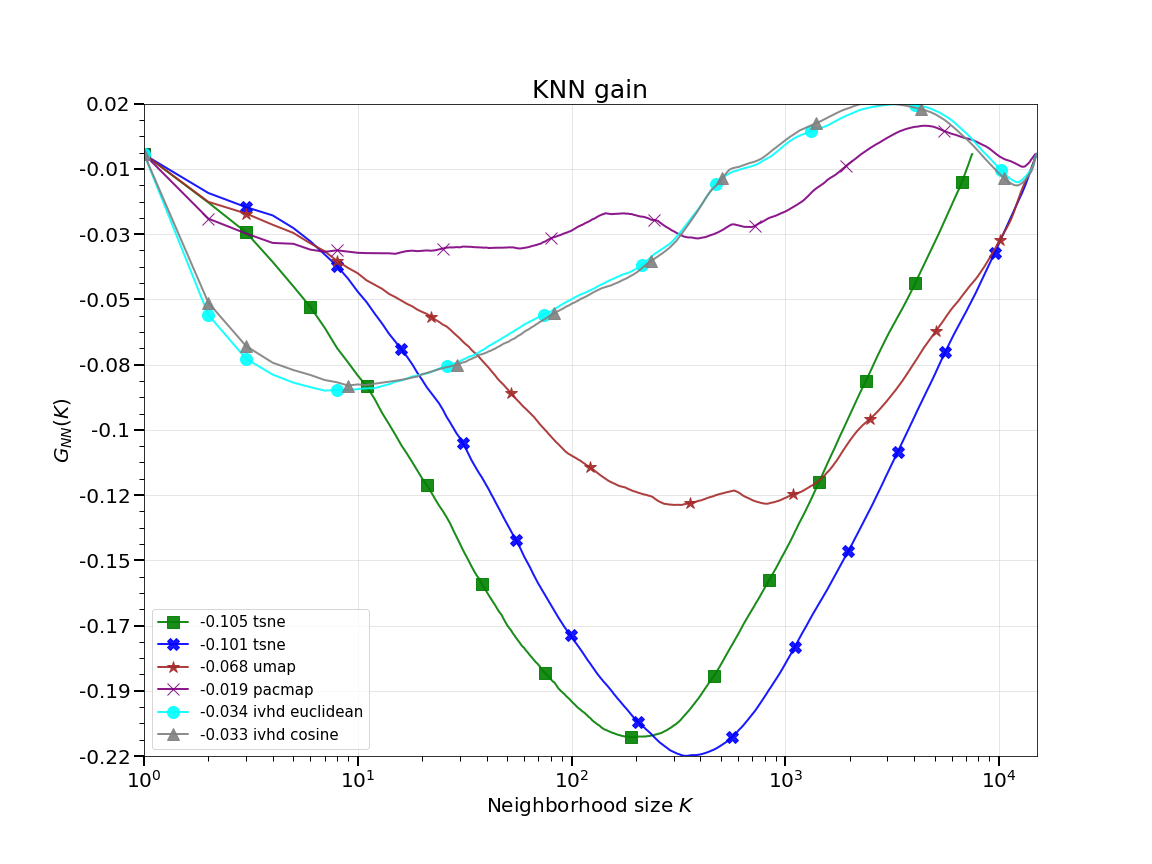
\includegraphics[width=\linewidth]{RCV Reuters/RCV-Reuters-knn-gain.png}
  \label{fig:sub2}
\end{subfigure}
\caption{DR quality and KNN gain for RCV Reuters}
\label{fig:test}
\end{figure}
Again, the metric indicates superior preservation of the local neighborhood by the t-SNE. Generally, IVHD behaves better and better when neighborhood size arises. KNN gain additionally enforces such a conclusion. Furthermore, PaCMAP results are consistent, and its embedding maintains a high level of mapping throughout the verified neighborhood size range. However, the key turns out to be global separation, where IVHD dominates.

\clearpage
\subsubsection{Co-ranking matrix}
\begin{figure}[h]
    \centering
    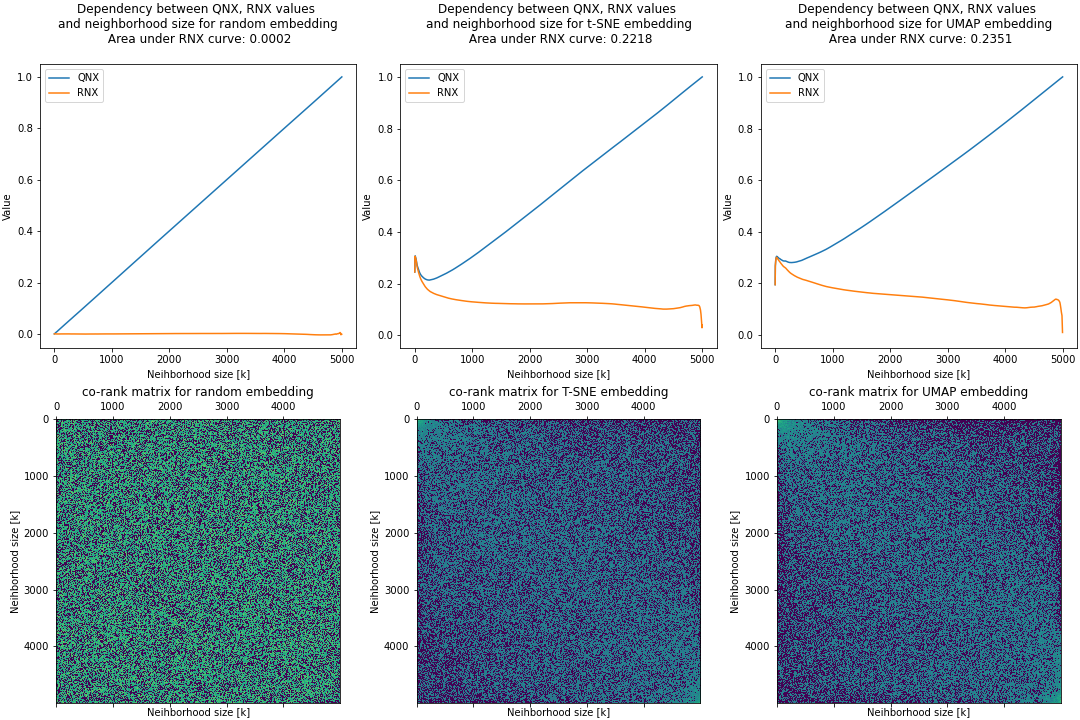
\includegraphics[width=0.95\textwidth]{RCV Reuters/RCV-Reuters-co-rank-matrix-part-1.png}
    \caption{Co-ranking matrix-based metrics. \\ Results for RCV Reuters embeddings using random embedding, t-SNE and UMAP.}
\end{figure}

\clearpage
\begin{figure}[h]
    \centering
    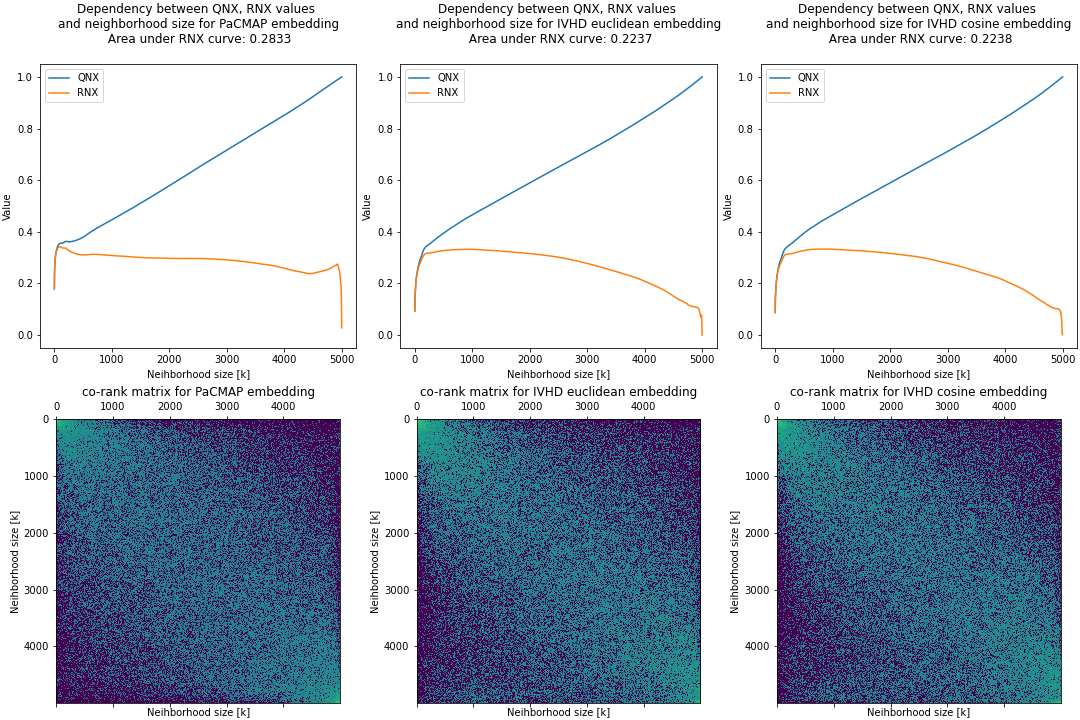
\includegraphics[width=0.95\textwidth]{RCV Reuters/RCV-Reuters-co-rank-matrix-part-2.png}
    \caption{Co-ranking matrix-based metrics. \\ Results for RCV Reuters embeddings using PaCMAP and IVHD.}
\end{figure}
The metric characterizes PaCMAP as a method that has practically retained an almost constant level of quality and mapping for the sets of the analyzed neighbors. Its profit is visible for the increasing number of neighbors compared to the results of other methods.

\clearpage
\subsubsection{Shepard diagrams}
\begin{figure}[h]
    \centering
    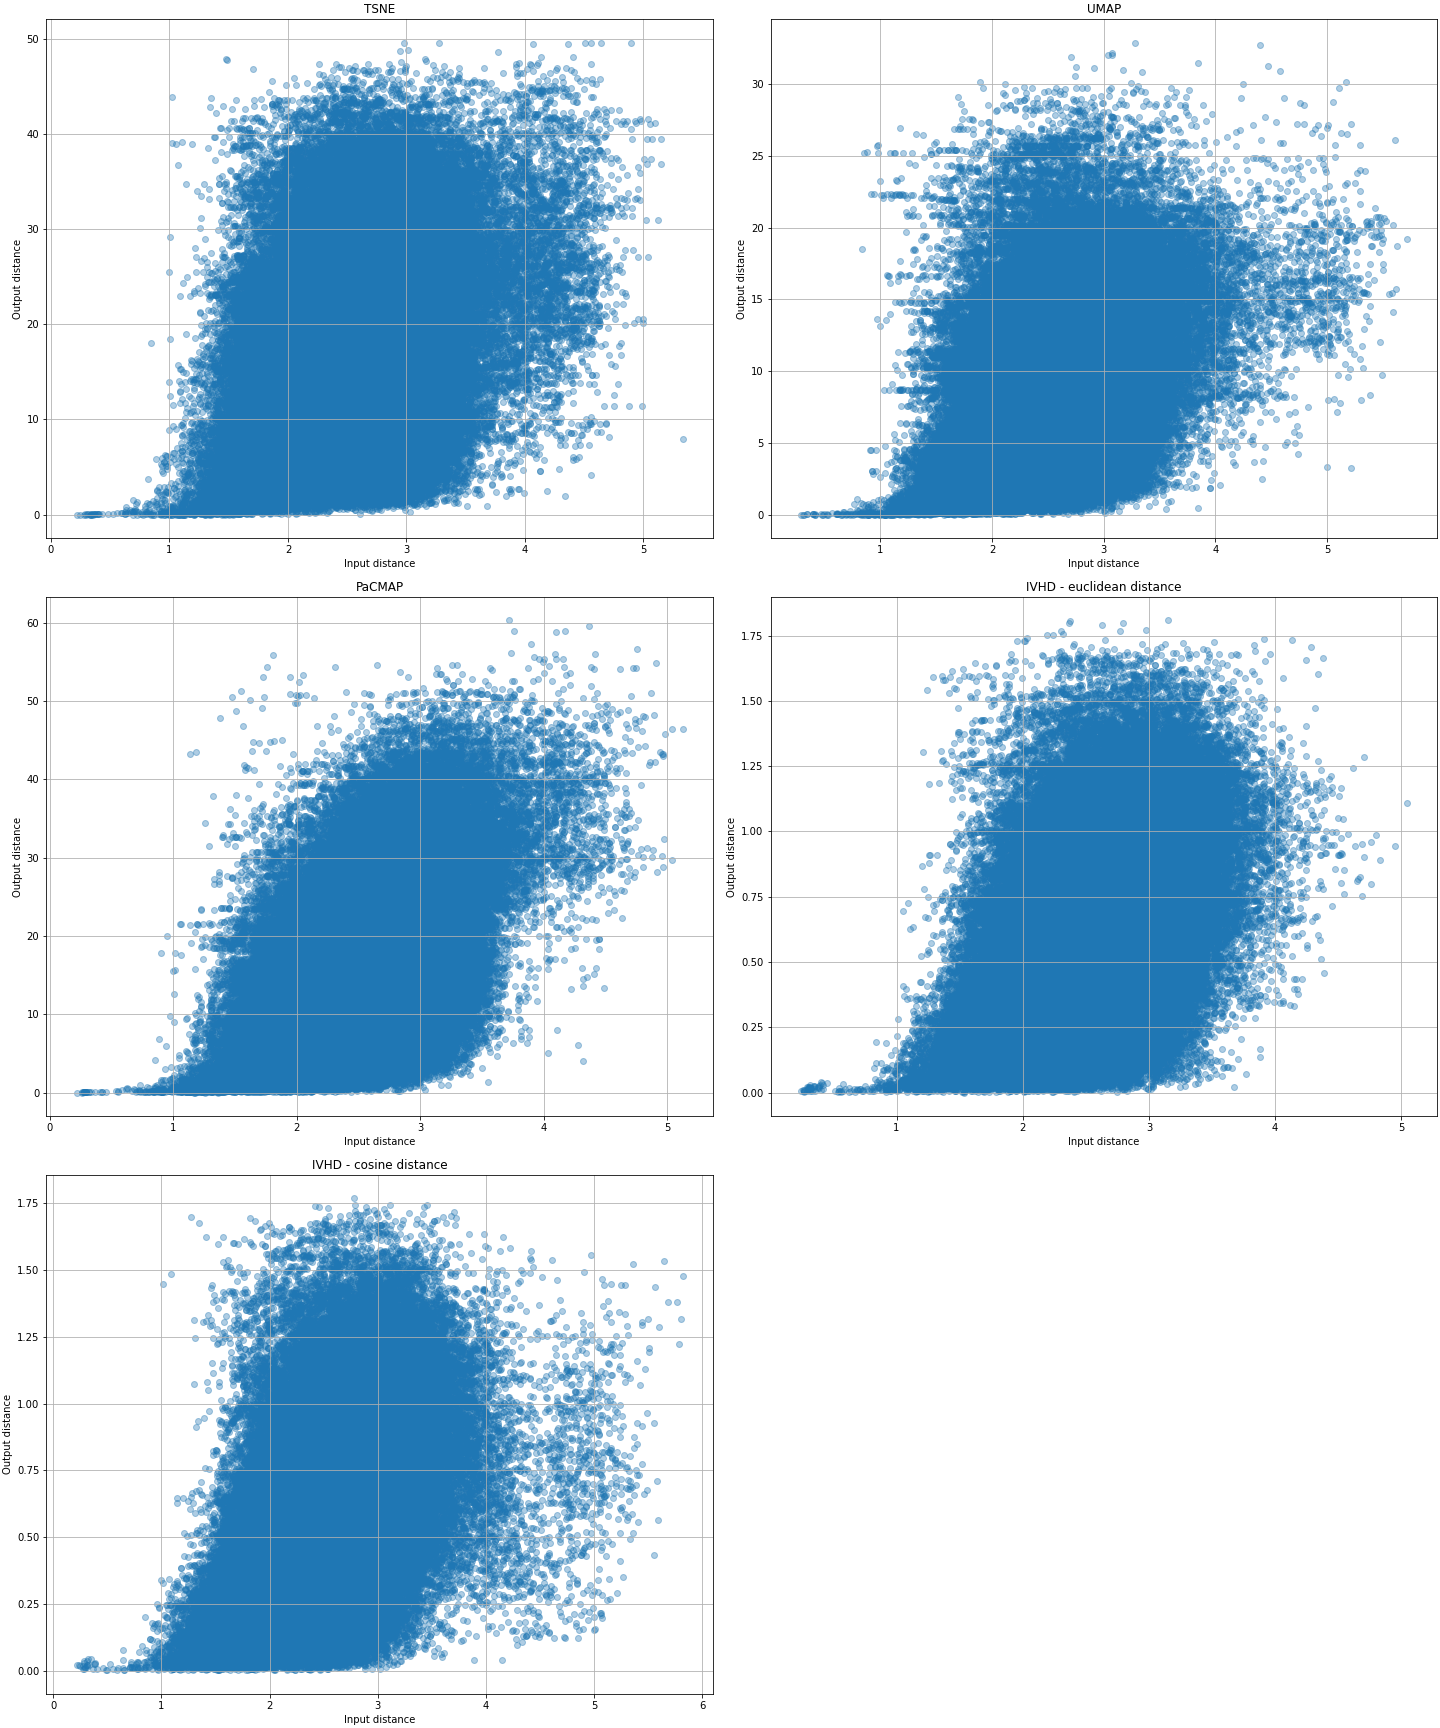
\includegraphics[width=0.8\textwidth]{RCV Reuters/RCV-Reuters-shepard-diagrams.png}
    \caption{Shepard diagrams of RCV Reuters embeddings using t-SNE, UMAP, PaCMAP and IVHD.}
\end{figure}
The Shepard diagrams for PaCMAP and IVHD euclidean represent points centered around a straight line quite well. The greater the input distance, the more difficult it is to rescale it in a space with reduced dimensions. Therefore, for all methods (especially t-SNE, UMAP, and IVHD cosine) and high input distance values, a significant number of points are separated from the group.

\clearpage

\subsubsection{Trustworthiness}
\begin{table}[h]
\centering
\caption{Trustworthiness with euclidean metric for pairwise distances. \\
Results for RCV Reuters embeddings using t-SNE, UMAP, PaCMAP and IVHD.}
\begin{tabular}{|c|c|c|c|c|c|}
\hline
\textbf{K} & \textbf{t-SNE} & \textbf{UMAP} & \multicolumn{1}{l|}{\textbf{PaCMAP}} & \multicolumn{1}{l|}{\textbf{IVHD euclidean}} & \multicolumn{1}{l|}{\textbf{IVHD cosine}} \\ \hline
5          & 0.907          & 0.915         & 0.935                                & 0.862                                        & 0.864                                     \\ \hline
15         & 0.847          & 0.883         & 0.919                                & 0.854                                        & 0.855                                     \\ \hline
50         & 0.763          & 0.828         & 0.897                                & 0.845                                        & 0.845                                     \\ \hline
100        & 0.717          & 0.793         & 0.876                                & 0.834                                        & 0.834                                     \\ \hline
150        & 0.692          & 0.772         & 0.860                                & 0.830                                        & 0.830                                     \\ \hline
\end{tabular}
\centering
\end{table}

\begin{table}[h]
\centering
\caption{Trustworthiness with cosine metric for pairwise distances. \\
Results for RCV Reuters embeddings using t-SNE, UMAP, PaCMAP and IVHD.}
\begin{tabular}{|c|c|c|c|c|c|}
\hline
\textbf{K} & \textbf{t-SNE} & \textbf{UMAP} & \multicolumn{1}{l|}{\textbf{PaCMAP}} & \multicolumn{1}{l|}{\textbf{IVHD euclidean}} & \multicolumn{1}{l|}{\textbf{IVHD cosine}} \\ \hline
5          & 0.922          & 0.933         & 0.951                                & 0.884                                        & 0.884                                     \\ \hline
15         & 0.868          & 0.905         & 0.940                                & 0.877                                        & 0.878                                     \\ \hline
50         & 0.788          & 0.857         & 0.923                                & 0.870                                        & 0.870                                     \\ \hline
100        & 0.741          & 0.823         & 0.904                                & 0.861                                        & 0.862                                     \\ \hline
150        & 0.714          & 0.801         & 0.890                                & 0.857                                        & 0.858                                     \\ \hline
\end{tabular}
\end{table}
In the case of t-SNE and UMAP, we can observe the relatively large variability of the range of trustworthiness values for the examined number of neighbors compared to the trustworthiness of other methods - PaCMAP and IVHD. Therefore, PaCMAP and IVHD are definitely at the forefront in terms of local structure preservation. Additionally, the latter can be favored by the same quality of trustworthiness, regardless of the number of neighbors in a given range.


\subsubsection{Spearman correlation-based metric}
\begin{table}[h]
\centering
\caption{Spearman correlation-based metric. \\ Results for RCV Reuters embeddings using t-SNE, UMAP, PaCMAP and IVHD.}
\begin{tabular}{|c|c|l|l|l|}
\hline
\textbf{t-SNE} & \textbf{UMAP} & \textbf{PaCMAP}            & \textbf{IVHD euclidean}    & \textbf{IVHD cosine}       \\ \hline
0.388          & 0.397         & \multicolumn{1}{c|}{0.541} & \multicolumn{1}{c|}{0.537} & \multicolumn{1}{c|}{0.536} \\ \hline
\end{tabular}
\end{table}
The metric based on the Spearman correlation confirms the conclusions drawn based on the trustworthiness metric. The PaCMAP and IVHD methods obtained the best results of similarity of the distances in both dimensionalities.

\clearpage
\section{Summary and Conclusions}
In this section, the results of the metrics obtained for the analyzed sets and the methods of data dimensionality reduction were summarized and compared. Additionally, this section was enriched with overall conclusions about high dimensional data visualization.

\begin{table}[h]
\centering
\caption{Summary of metrics results for MNIST.}
\begin{tabular}{|l|l|
>{\columncolor[HTML]{9AFF99}}c |l|
>{\columncolor[HTML]{FFCCC9}}l |
>{\columncolor[HTML]{FFCCC9}}l |}
\hline
\textbf{Metric}                          & \textbf{t-SNE}         & \multicolumn{1}{l|}{\cellcolor[HTML]{9AFF99}\textbf{UMAP}} & \textbf{PaCMAP}        & \textbf{\begin{tabular}[c]{@{}l@{}}IVHD \\ euclidean\end{tabular}} & \textbf{\begin{tabular}[c]{@{}l@{}}IVHD \\ cosine\end{tabular}} \\ \hline
Distance matrix-based metric             &                        & X                                                          &                        &                                                                    &                                                                 \\ \hline
Distance matrix-based metric with KMeans &                        & X                                                          &                        &                                                                    &                                                                 \\ \hline
DR quality and KNN gain                  &                        & X                                                          & \multicolumn{1}{c|}{X} &                                                                    &                                                                 \\ \hline
Co-ranking matrix                        & \multicolumn{1}{c|}{X} & \multicolumn{1}{l|}{\cellcolor[HTML]{9AFF99}}              &                        &                                                                    &                                                                 \\ \hline
Sheppard diagram                         &                        & X                                                          & \multicolumn{1}{c|}{X} &                                                                    &                                                                 \\ \hline
Trustworthiness                          &                        & X                                                          & \multicolumn{1}{c|}{X} &                                                                    &                                                                 \\ \hline
Spearman correlation-based metric        &                        & X                                                          & \multicolumn{1}{c|}{X} &                                                                    &                                                                 \\ \hline
\end{tabular}
\end{table}

\begin{table}[h]
\centering
\caption{Summary of metrics results for 20 News Groups.}
\begin{tabular}{|l|l|
>{\columncolor[HTML]{FFFFFF}}c |
>{\columncolor[HTML]{FFCCC9}}l |
>{\columncolor[HTML]{9AFF99}}c |
>{\columncolor[HTML]{FFCCC9}}l |}
\hline
\textbf{Metric}                          & \textbf{t-SNE}         & \multicolumn{1}{l|}{\cellcolor[HTML]{FFFFFF}\textbf{UMAP}} & \textbf{ISOMAP}                               & \multicolumn{1}{l|}{\cellcolor[HTML]{9AFF99}\textbf{\begin{tabular}[c]{@{}l@{}}IVHD \\ euclidean\end{tabular}}} & \textbf{\begin{tabular}[c]{@{}l@{}}IVHD \\ cosine\end{tabular}} \\ \hline
Distance matrix-based metric             &                        &                                                            &                                               & X                                                                                                               & \multicolumn{1}{c|}{\cellcolor[HTML]{FFCCC9}}                   \\ \hline
Distance matrix-based metric with KMeans &                        &                                                            &                                               & X                                                                                                               & \multicolumn{1}{c|}{\cellcolor[HTML]{FFCCC9}}                   \\ \hline
DR quality and KNN gain                  &                        &                                                            & \multicolumn{1}{c|}{\cellcolor[HTML]{FFCCC9}} & X                                                                                                               &                                                                 \\ \hline
Co-ranking matrix                        & \multicolumn{1}{c|}{X} & \multicolumn{1}{l|}{\cellcolor[HTML]{FFFFFF}}              &                                               & \multicolumn{1}{l|}{\cellcolor[HTML]{9AFF99}}                                                                   &                                                                 \\ \hline
Sheppard diagram                         &                        &                                                            & \multicolumn{1}{c|}{\cellcolor[HTML]{FFCCC9}} & X                                                                                                               &                                                                 \\ \hline
Trustworthiness                          &                        &                                                            & \multicolumn{1}{c|}{\cellcolor[HTML]{FFCCC9}} & X                                                                                                               &                                                                 \\ \hline
Spearman correlation-based metric        & \multicolumn{1}{c|}{X} & X                                                          & \multicolumn{1}{c|}{\cellcolor[HTML]{FFCCC9}} & \multicolumn{1}{l|}{\cellcolor[HTML]{9AFF99}}                                                                   &                                                                 \\ \hline
\end{tabular}
\end{table}


\begin{table}[h]
\centering
\caption{Summary of metrics results for RCV Reuters.}
\begin{tabular}{|l|
>{\columncolor[HTML]{FFCCC9}}l |
>{\columncolor[HTML]{FFCCC9}}c |
>{\columncolor[HTML]{FFFFFF}}c |
>{\columncolor[HTML]{9AFF99}}c |
>{\columncolor[HTML]{9AFF99}}c |}
\hline
\textbf{Metric}                          & \textbf{t-SNE}                                & \multicolumn{1}{l|}{\cellcolor[HTML]{FFCCC9}\textbf{UMAP}} & \multicolumn{1}{l|}{\cellcolor[HTML]{FFFFFF}\textbf{PaCMAP}} & \multicolumn{1}{l|}{\cellcolor[HTML]{9AFF99}\textbf{\begin{tabular}[c]{@{}l@{}}IVHD \\ euclidean\end{tabular}}} & \multicolumn{1}{l|}{\cellcolor[HTML]{9AFF99}\textbf{\begin{tabular}[c]{@{}l@{}}IVHD \\ cosine\end{tabular}}} \\ \hline
Distance matrix-based metric             &                                               &                                                            &                                                              & X                                                                                                               & X                                                                                                            \\ \hline
Distance matrix-based metric with KMeans &                                               &                                                            &                                                              & X                                                                                                               & X                                                                                                            \\ \hline
DR quality and KNN gain                  &                                               &                                                            &                                                              & X                                                                                                               & X                                                                                                            \\ \hline
Co-ranking matrix                        & \multicolumn{1}{c|}{\cellcolor[HTML]{FFCCC9}} & \multicolumn{1}{l|}{\cellcolor[HTML]{FFCCC9}}              & X                                                            &                                                                                                                 &                                                                                                              \\ \hline
Sheppard diagram                         &                                               &                                                            & X                                                            & X                                                                                                               & X                                                                                                            \\ \hline
Trustworthiness                          &                                               &                                                            & X                                                            & X                                                                                                               & X                                                                                                            \\ \hline
Spearman correlation-based metric        & \multicolumn{1}{c|}{\cellcolor[HTML]{FFCCC9}} &                                                            & X                                                            & X                                                                                                               & X                                                                                                            \\ \hline
\end{tabular}
\end{table}

\clearpage
According to metrics value, UMAP gave the best results for the MNIST dataset in the context of both local and global separation, PaCMAP also gives reasonable results. In this case, IVHD gave the worst effects, none of the examined metrics showed its superiority over other ones. In the case of 20 News Group, IVHD with Euclidean distance metric gives considerably better results than other methods, but in contrast, IVHD with cosine distance metric gives the worst embedding. ISOMAP also acts poorly in this case. For the RCV Reuters, the IVHD method gives the best results, and PaCMAP also gives decent results. None of the considered metrics showed domination of t-SNE or UMAP in the case of this dataset. Multiple metrics are available to assess the quality of dimensionality reduction techniques. The vast majority of them relate to local separation. Unfortunately, not all data sets allow for an intuitive assessment of the meaningfulness of the resulting clusters. MNIST is a perfect example of the one with very high interpretability. Therefore it is worth using diversified metrics that allow for more in-depth analysis and provide a strong foundation for formulating justified assessments. The use of various methods, the inspection of visualizations supported by the conclusions drawn from metrics interpretation, allows noticing the challenges facing this field. A visualization is undoubtedly a powerful tool where each DR technique can show its advantages depending on the highlighted goal to achieve. Finally, one of the most vital issues is the appropriate parameterization of methods. It undoubtedly affects the quality of dimensionality reduction and can radically change the obtained visualizations. Unfortunately, there is no one unique method that works best for each data set. Evaluation and verification should be made to match the one appropriate to the issue under consideration.
\\ \\
The source code and complete visualizations are available at the following location: \\
\url{https://github.com/Smendowski/data-embedding-and-visualization}

\clearpage
\printbibliography
\end{document}